\documentclass[11pt,letterpaper]{article}

\usepackage[T1]{fontenc}
\usepackage{lmodern}
\usepackage{textcomp}
\usepackage[margin=1in]{geometry}
\usepackage{amsmath,amssymb}
\usepackage{graphicx}
\usepackage{booktabs}
\usepackage{tabularx}
\usepackage{microtype}
\usepackage{xcolor}
\usepackage[font=small,labelfont=bf]{caption}
\usepackage{cite}
\usepackage{hyperref}

\makeatletter
\g@addto@macro\UrlBreaks{\do\/\do\-\do\_\do\.\do\a\do\b\do\c\do\d\do\e\do\f\do\g\do\h\do\i\do\j\do\k\do\l\do\m\do\n\do\o\do\p\do\q\do\r\do\s\do\t\do\u\do\v\do\w\do\x\do\y\do\z}
\makeatother

\hypersetup{
    colorlinks=true,
    linkcolor=blue!80!black,
    citecolor=blue!80!black,
    urlcolor=blue!80!black
}

\setcounter{secnumdepth}{0}
\renewcommand{\topfraction}{0.95}
\renewcommand{\bottomfraction}{0.95}
\renewcommand{\textfraction}{0.05}
\renewcommand{\floatpagefraction}{0.75}
\setcounter{topnumber}{3}
\setcounter{bottomnumber}{3}
\setcounter{totalnumber}{4}

\title{\textbf{Verifiable Agentic Science on Public Infrastructure}}

\author{
  Dannon Baker$^{1,6}$, Scott Cain$^{2,6}$, Marius van den Beek$^{2,6}$, John Chilton$^{2,6}$,\\
  Danielle Callan$^{2,6}$, Steven Weaver$^{3}$, Nate Coraor$^{2,6}$, Kelsey Beavers$^{4}$,\\
  Michael C. Schatz$^{1,6}$, Bj\"orn Gr\"uning$^{5,6,7}$, Sergei L. Kosakovsky Pond$^{3,*}$, and Anton Nekrutenko$^{2,6,*}$\\[0.8em]
  \small $^{1}$Department of Biology, Johns Hopkins University, Baltimore, MD, USA\\
  \small $^{2}$Department of Biochemistry and Molecular Biology, Penn State University, University Park, PA, USA\\
  \small $^{3}$Institute for Genomics and Evolutionary Medicine, Department of Biology,\\
  \small Temple University, Philadelphia, PA, USA\\
  \small $^{4}$Texas Advanced Computing Center, The University of Texas at Austin, Austin, TX, USA\\
  \small $^{5}$Department of Computer Science, University of Freiburg, Freiburg, Germany\\
  \small $^{6}$\href{https://galaxyproject.org}{galaxyproject.org}\\
  \small $^{7}$\href{https://usegalaxy.eu}{usegalaxy.eu}\\[0.3em]
  \small $^{*}$Correspondence: \texttt{spond@temple.edu}, \texttt{anton@nekrut.org}
}

\date{}

\begin{document}

\maketitle

\begin{abstract}
Autonomous coding agents can run complex biological analyses from a single prompt, yet running them on personal machines threatens scientific reliability. In local shells, agents invent conflicting pipelines, write disposable scripts, hit hardware limits, and leave no verifiable trail. Here we build something that has never existed: a shared public plane where agents conduct data analysis responsibly at scale. By connecting any language-model agent---or Orbit, our dedicated research workbench---to public Galaxy cyberinfrastructure via community skills, the Model Context Protocol, Workflow Foundry, and BRC-Analytics, we route compute-intensive steps onto national supercomputers and record the complete lineage in a shareable research notebook. We evaluate this architecture across 47 published benchmark datasets (46 distinct biological cohorts) and one novel structural phylogenomics study spanning spatial transcriptomics, pathogen and vector functional genomics, and epidemiology. Complete workflow provenance uncovers unstated statistical pooling and post-processing rules in published fungal and mosquito studies alongside an undocumented 1,000-cell tutorial subset choice in a recent \textit{Nature} Paper2Agent spatial transcriptomics benchmark. Beyond auditing past work, the platform enables cutting-edge discovery at scale. It collapses 146 fragmented \textit{Plasmodium vivax} antigen subfamilies into 73--76 structural classes across local CPU and remote NVIDIA A100 GPU runs---with 21 three-continent classes holding over 97\% of the repertoire---and dates 42 pathogen epidemic alignments in seconds of core manifold computation per cohort rather than hours to days of Bayesian Markov chain Monte Carlo sampling. Our system unites the speed of autonomous agents with strict reproducibility, showing what future science can achieve on shared public infrastructure.
\end{abstract}

\section{Introduction}

Across all scientific domains, LLM-powered agents formulate hypotheses, build analytical pipelines, execute code, and draft complete research manuscripts \cite{boiko2023, chemcrow2024, virtuallab2025, aiscientist2024, kosmos2025, huang2025biomni}. Recognizing these capabilities, academic and corporate laboratories have created purpose-built research environments such as Google's AI Co-Scientist to coordinate autonomous research \cite{coscientist2026}. Yet domain platforms cannot match the rapid development velocity, model optimizations, and tooling ecosystems powering general-purpose agent harnesses from the major artificial intelligence providers---Google, Anthropic, and OpenAI. At our own research institutions, we have watched numerous graduate students, postdocs, and PIs (even those who are AI-averse) adopt these agentic tools, become hooked, and stop analyzing data in any other way. This quickly makes general agent harnesses the primary working environment for modern computational research.

This rapidly widening use of agentic tools in science is equally thrilling and terrifying. The thrill comes from the speed and seemingly unlimited number of possibilities that suddenly became available to any researcher. The terror comes from a completely new set of scientific challenges that are not immediately apparent but will become severe as agentic science becomes the new norm. First, provenance tracking is largely absent. As unsupervised agents iterate, they generate ephemeral shell scripts, unversioned intermediate tables, and temporary scratch files. These ad-hoc artifacts vanish as soon as the session closes, and few have the proper version control skills and discipline to keep the full record. Scientific research requires that every analytical operation, tool version, and parameter choice be formalized into an immutable, shareable record so that colleagues can inspect, verify, and reproduce the complete computational trajectory. Second, autonomous agents require community-curated skills and standardized, high-quality bioinformatics tools. Rather than improvising custom scripts from unvetted online snippets, agents must make analytical decisions guided by verified computational protocols and validated tool specifications that function across different agent harnesses. Third, the agentic revolution does not change the need for infrastructure access. While modern laptops handle exploratory scripting effectively, production biological workflows---such as large-scale genome assembly, analyses of large multi-sample datasets, or deep learning inference---demand high-performance computing clusters with hundreds of processor cores, massive memory allocations, and dedicated hardware accelerators. Installing autonomous agent harnesses directly onto shared institutional supercomputers violates facility security policies and remains administratively unsustainable.

For over twenty years, the Galaxy platform has provided open, reproducible cyberinfrastructure to life scientists worldwide \cite{galaxy2024}. It now serves as an ideal agentic plane to address these challenges. First, it provides a universal compute abstraction that schedules complex, containerized analytical workloads across heterogeneous institutional clusters, national supercomputing allocations, and commercial clouds without requiring interactive login credentials, private keys, or command-line administrative access. Second, Galaxy's web interface and history system serve as an ideal artifact display mechanism. Every analytical step, parameter choice, and intermediate dataset is recorded within an immutable directed acyclic graph that investigators and their collaborators can inspect, audit, visualize, and re-execute with a single click. Third, the platform supplies the definitive scientific knowledge base. The Intergalactic Utilities Commission maintains thousands of vetted, containerized tool wrappers \cite{iuc2026, biocontainers2017}, the Intergalactic Workflow Commission curates standardized analytical pipelines \cite{iwc2026}, and the Galaxy Training Network provides hundreds of peer-reviewed, step-by-step procedural tutorials \cite{batut2018, hiltemann2023}. Finally, the Workflow Foundry translates external bioinformatics knowledge---including Nextflow pipelines and published methods---into structured agentic skills that guide autonomous execution across Galaxy cyberinfrastructure \cite{foundry2026}. Galaxy grounds autonomous language models in transparent, reproducible, and vendor-agnostic scientific infrastructure.

Here we demonstrate our platform across seven biological investigations encompassing 48 empirical evaluations. These reproduce 47 published datasets (46 distinct cohorts: 5 transcriptomic, epigenomic, single-cell, and spatial studies plus 42 pathogen alignments across 41 outbreaks from 37 publications) and conduct a novel three-genome structural phylogenomics analysis of malaria antigens. In spatial transcriptomics, Orbit packages a published conformal-prediction pipeline as User-Defined Tools on UseGalaxy.org, matches local point predictions to floating-point precision ($r = 1.0000$, $\Delta_{\max} < 10^{-15}$) on the 1,000-cell tutorial subset, and scales the workflow to the full 5,613-cell reference cohort to triple prediction-to-measurement correlation ($r = 0.0861$ to $0.2553$). Across bacterial, fungal, and mosquito vector genomics, autonomous workflows compiled from published methods and community skills reproduce multi-sample transcriptomic, ATAC-seq, and single-cell atlases while uncovering unstated statistical pooling, annotation mismatches, and post-processing rules. In structural phylogenomics, the agent builds unprivileged User-Defined Tools to execute deep-learning protein language models across local and remote GPU/CPU resources, collapsing 146 fragmented \textit{Plasmodium vivax} antigen subfamilies into 73 (local CPU reference) to 76 (remote A100 GPU and 32-core CPU) structural classes, with 21 three-continent classes holding over 97\% of the repertoire. In genomic epidemiology, the platform automates emergence dating across 42 published pathogen epidemic alignments, evaluating tree-free molecular clock estimates against published Bayesian benchmarks in seconds per alignment. Across all seven investigations, every analytical step, containerized tool, and intermediate dataset is documented as an immutable history on public cyberinfrastructure.

\section{Results}

\subsection{Advanced models propose vastly different analysis plans ...}

Today many biological researchers discover how seemingly easy it is to conduct data analysis with agents. Suppose a student is given a task of analyzing RNA-seq data by an advisor. The student is adventurous enough to try to use one of the widely advertised agents. The student uploads data, explains to the agent the experimental design, and asks it to propose an analysis plan (note that planning is not a widely adopted discipline in biomedical research and that appropriate use of agents requires significant changes to the present curriculum). How does the student know that the proposed plan is good? How would the student choose among possibilities proposed by an agent? To illustrate this problem we asked 30 agents (10 for each of Anthropic, OpenAI, and Google, respectively) to propose reanalysis plans for a paper (because we know what the expected outcome should be) describing a published transcriptomic study (PMC12804731) \cite{vyklicka2026}. The 30 plans fragmented into 18 distinct eight-step plans (Figure~\ref{fig:agent_trajectories}). Even when restricted to the five result-changing biological and statistical steps (reference assembly, read aligner, quantified genomic feature, ribosomal RNA handling, and differential expression model scope), the plans formed 11 distinct five-step plans. The most common five-step plan was shared by only 7 of the 30 plans, meaning 23 of 30 diverged from the most common plan and 29 of 30 diverged from the published study's exact workflow. These conflicting choices across reference genomes, read strandedness, and statistical sample pooling also result in dramatic changes in resource requirements, as shown in Supplementary Table~\ref{tab:agent_resources}. 

\begin{figure}[!htbp]
\centering
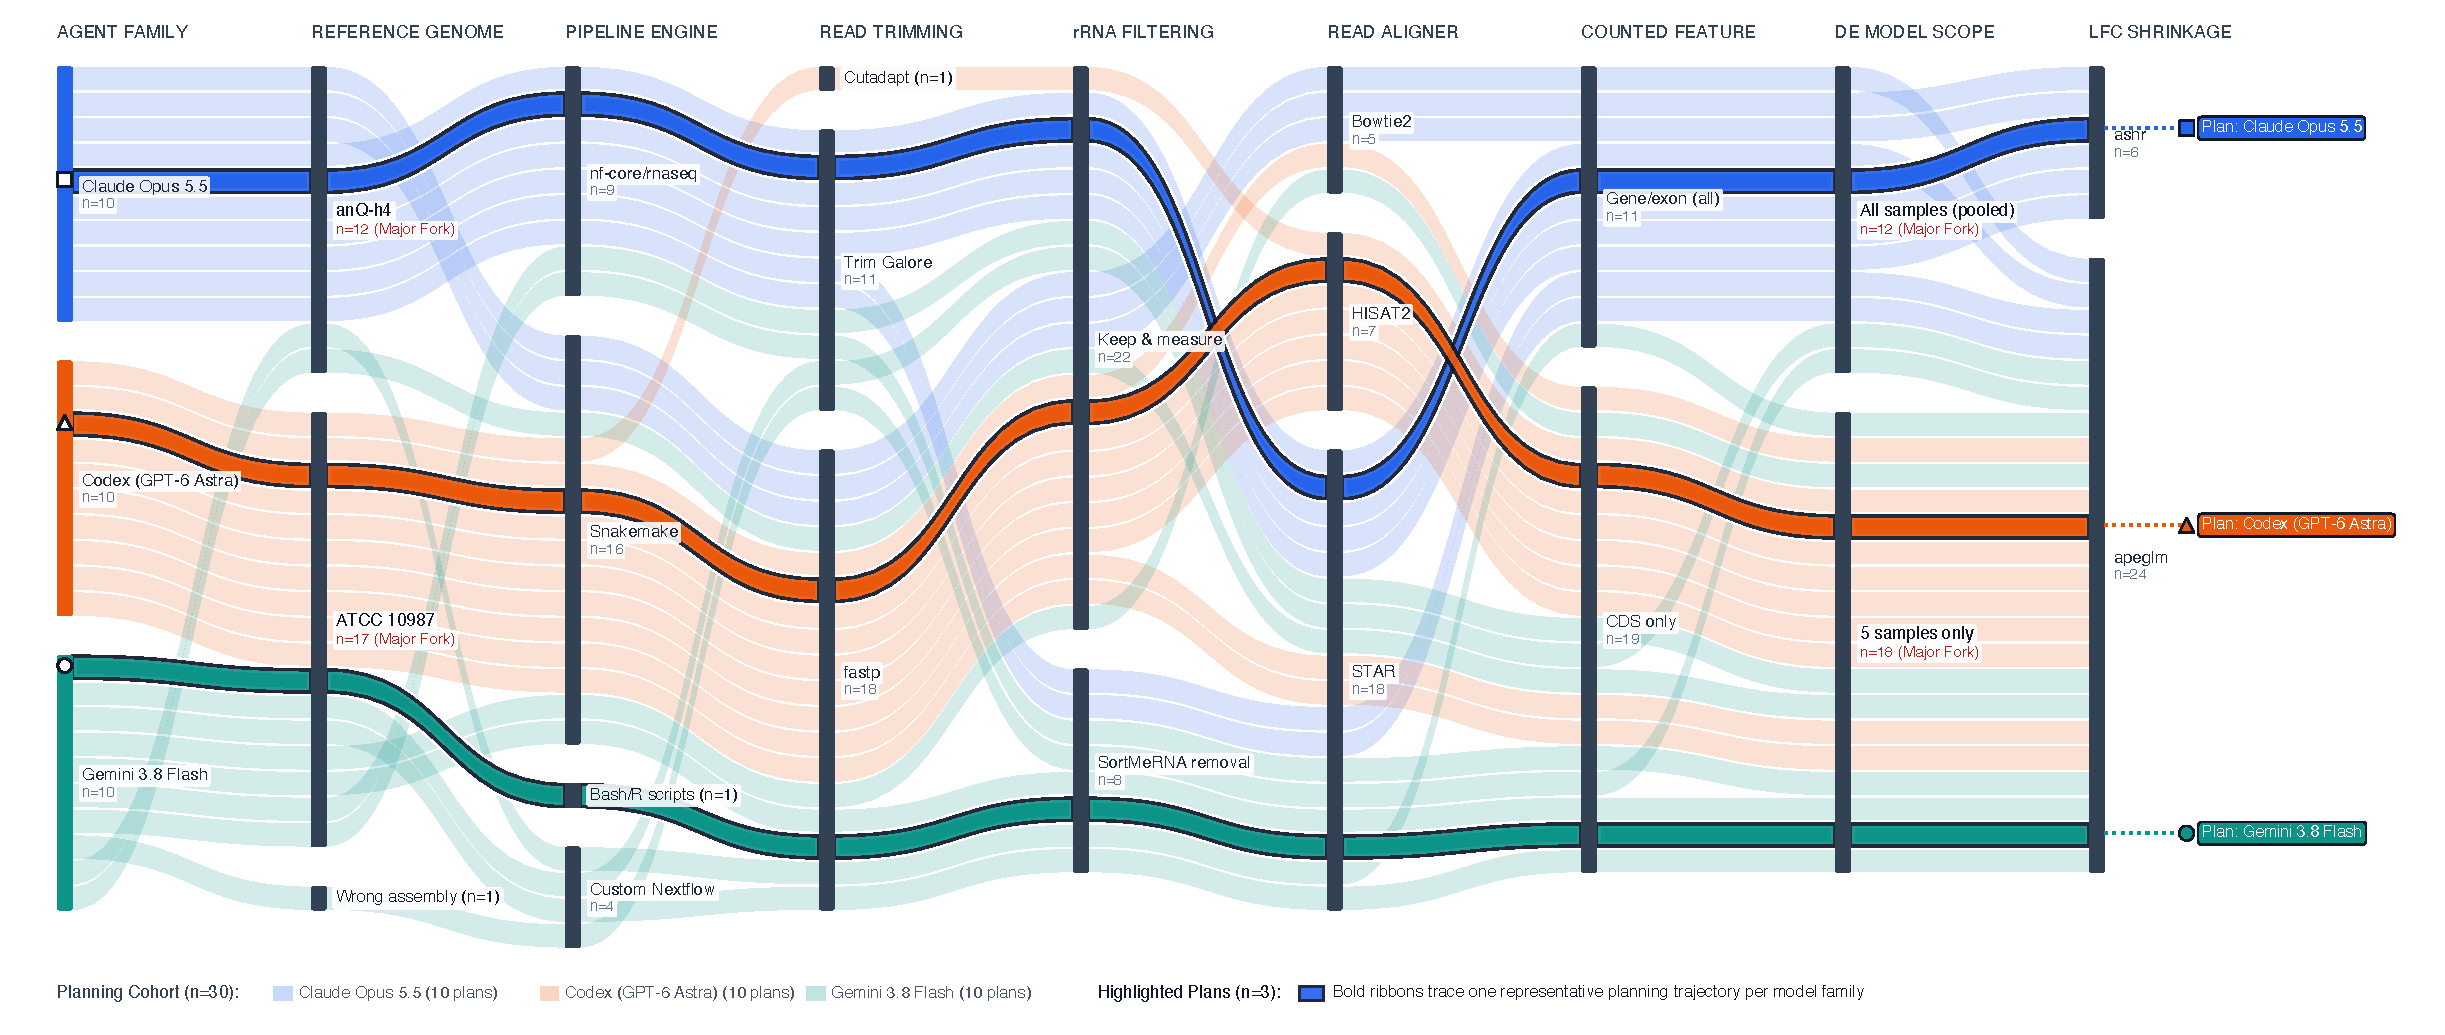
\includegraphics[width=0.90\textwidth]{figures/figure1_agent_trajectories.pdf}
\caption{\textbf{Combinatorial divergence in autonomous agent planning trajectories.} 
Thirty isolated large language model agents (ten Claude Opus 5.5, ten OpenAI Codex running GPT-6 Astra, and ten Google Gemini 3.8 Flash via Antigravity) were tasked with planning an end-to-end replication of \textit{Bacillus cereus} transcriptomic responses to carbohydrate supplementation (PMC12804731) without access to Galaxy cyberinfrastructure. Plans were evaluated across three foundation model families and eight sequential analytical steps: reference genome assembly, pipeline workflow engine, read trimming software, ribosomal RNA depletion strategy, read aligner, quantified genomic feature, differential expression model scope, and log-fold-change shrinkage prior. Transparent background ribbons trace individual planning trajectories, colored by model family (blue for Claude Opus 5.5, orange for OpenAI Codex, and teal for Google Gemini 3.8 Flash). Bold highlighted ribbons trace one representative planning trajectory from each model family (square marker for Claude Opus 5.5, triangle marker for OpenAI Codex, and circle marker for Google Gemini 3.8 Flash). Node heights indicate the number of plans selecting each option. Unsupervised planning fragmented into 18 distinct eight-step plans and 11 distinct five-step plans across the five steps (reference genome, aligner, feature type, rRNA handling, and differential expression model scope) that directly alter final gene counts and significance calls. Across these five core steps, 23 of the 30 plans diverged from the most common five-step plan and 29 of 30 diverged from the published study's workflow.}
\label{fig:agent_trajectories}
\end{figure}

\subsection{... and leave a dusty trail of intermediates}

To test how autonomous agents perform in practice, we tasked one agent from each model family with executing an end-to-end reanalysis on dedicated local hardware (Supplementary Table~\ref{tab:agent_resources}). During live execution, each agent deviated further from its model family's most common plan as it adapted to local tool availability and archive metadata. Even so, all three recovered the expected biological signals (Figure~\ref{fig:agent_execution}). Each confirmed glucose repression of the enterotoxin subunit \textit{nheB}, induction of enterotoxin \textit{entFM}, and genomic absence of the \textit{hbl} operon. Yet beneath this biological concordance lay total computational divergence. The three platforms selected incompatible reference assemblies, different aligners, and conflicting statistical models. Their resource footprints varied by orders of magnitude (Supplementary Table~\ref{tab:agent_resources}). To bridge missing infrastructure, the agents generated twenty-six distinct custom scripts totaling over 1,200 lines of unversioned code (Supplementary Table~\ref{tab:agent_scripts}). Their engineering strategies differed fundamentally. Gemini executed three monolithic shell and R scripts with hardcoded local paths. Claude built nine wrapper scripts to drive containerized Nextflow pipelines. Codex engineered fourteen modular scripts to enforce memory limits and track pruned files. None of these custom scripts were portable or auditable beyond the machines where they ran. Each agent left behind an ephemeral debris field of temporary glue code, isolated environments, and unversioned logs. Autonomous agents can recover biological signals. They cannot produce shareable, permanent scientific records without a common cyberinfrastructure plane.

\begin{figure}[!htbp]
\centering
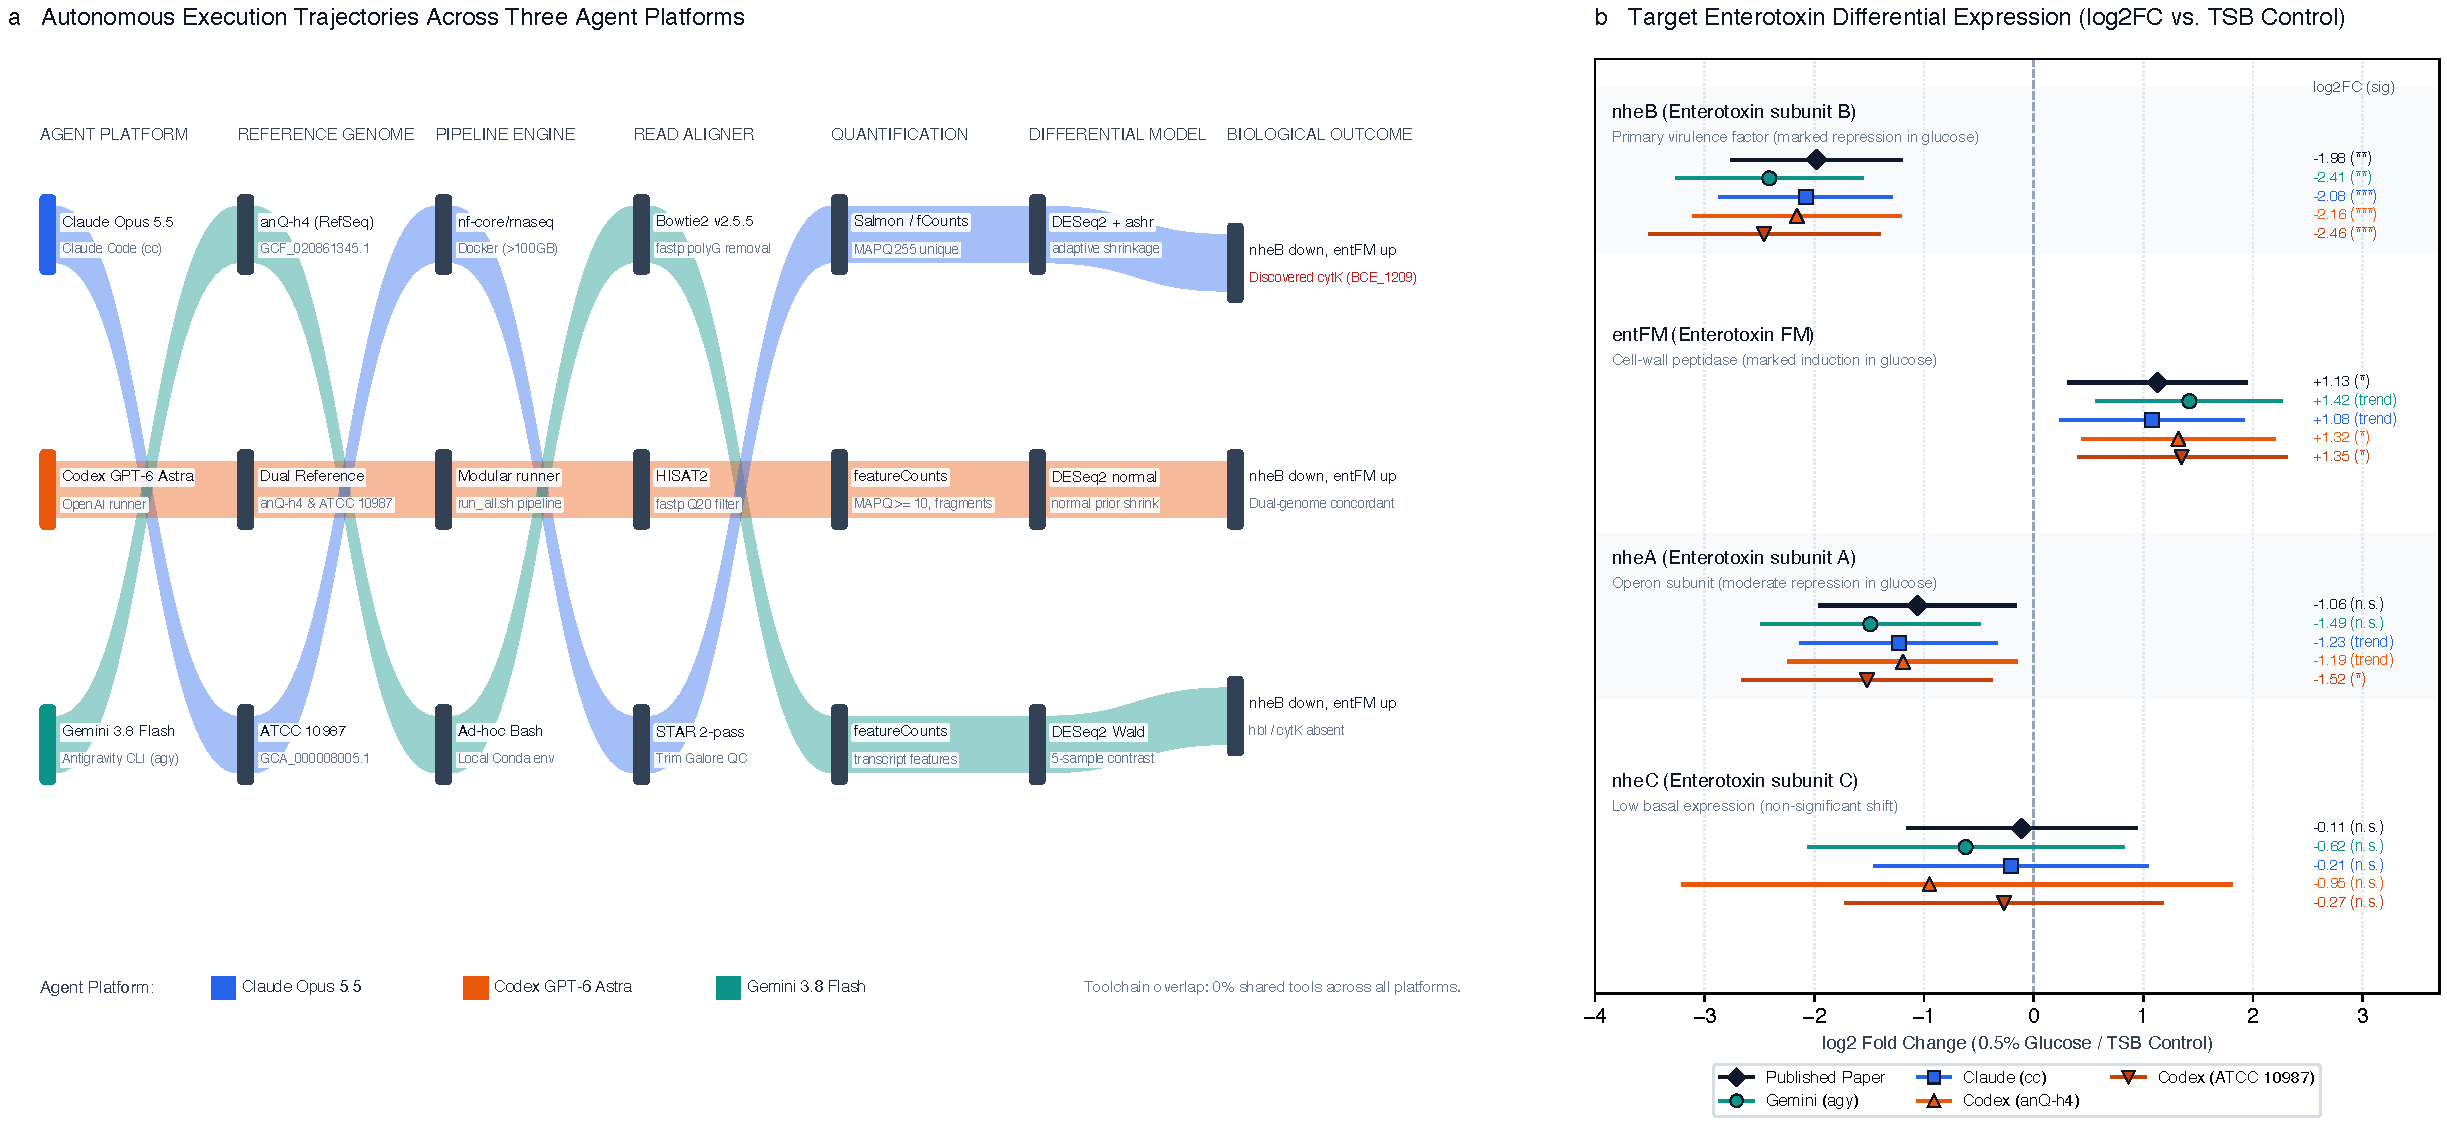
\includegraphics[width=\textwidth]{figures/figure2_agent_execution.pdf}
\caption{\textbf{Target enterotoxin differential expression and reference-assembly discordance across independent agent execution environments.} 
\textbf{A}, Estimated differential expression effect sizes ($\log_2\text{FC}$ and 95\% confidence intervals, $\log_2\text{FC} \pm 1.96 \cdot \text{lfcSE}$) and aligned adjusted $p$-values for target enterotoxin genes (\textit{nheB}, \textit{entFM}, \textit{nheA}, \textit{nheC}, and \textit{cytK2}) compared against the published benchmark (black diamonds, Vyklick{\'a} et al.\ \cite{vyklicka2026}, implied \textit{B.\ pacificus} anQ-h4). OpenAI Codex (orange and rust across both reference assemblies) and Antigravity (teal) report unshrunken DESeq2 Wald estimates, whereas Claude Code (blue, \texttt{nf-core/differentialabundance}) reports \texttt{ashr}-shrunken posterior estimates. For \textit{nheC} on \textit{B.\ pacificus} anQ-h4, where DESeq2 independent filtering sets $p_{\text{adj}}$ to \texttt{NA}, the table displays \texttt{NA} alongside the unadjusted Wald $p$-value. All three executed agent environments confirmed marked repression of \textit{nheB} and directional induction of \textit{entFM}. 
\textbf{B}, Reference-assembly discordance at the cytotoxin K (\textit{cytK2}, \texttt{BCE\_1209} / \texttt{BCE\_RS06135}) locus and enterotoxin repertoire recovery. Aligning to the sequenced isolate \textit{B.\ cereus} ATCC 10987 (\texttt{GCF\_000008005.1} / \texttt{GCA\_000008005.1}) in Claude Code and Codex recovered active baseline \textit{cytK2} transcription across all libraries (548--1,420 raw read pairs per library, mean 797, DESeq2 $\text{baseMean} = 831$, $\log_2\text{FC} = +0.58$, $p_{\text{adj}} = 0.43$). Aligning against \textit{B.\ pacificus} anQ-h4 left \textit{cytK2} undetected because the assembly lacks the \textit{cytK2} locus.}
\label{fig:agent_execution}
\end{figure}

\clearpage
\subsection{Agentic science on public infrastructure: The Galactic plane}

The benchmarking results above highlight the core problems of unassisted agentic science: conflicting and inconsistent analytical trajectories, unversioned glue code, and the limits of local hardware (Figures~\ref{fig:agent_trajectories} and~\ref{fig:agent_execution}). To produce trustworthy and verifiable results, agents need field-specific guidance and shared infrastructure (Figure~\ref{fig:architecture}). Domain skills and the Model Context Protocol (MCP) establish essential guardrails (Figure~\ref{fig:architecture}, Panel 2) \cite{galaxymcp2026, galaxyskills2026} by following community-curated analysis pathways and preferring validated tool invocations to generating transient code. But agents also need a uniform, shared execution engine for three reasons. First, compute scale and access: a modern laptop can process large amounts of data, but memory-intensive aligners like STAR \cite{dobin2013} quickly tax local memory and storage when run serially across multi-sample cohorts on a personal machine. Making agentic science accessible also requires accounting for researchers who lack powerful local hardware. Second, tools impossible to run locally: methods like, for example, AlphaGenome \cite{alphagenome2025}, Logan \cite{logan2024}, or LexicMap \cite{lexicmap2025} require massive indices or large models that no workstation can host. Third, and this is critical: reproducibility. One can argue that agentic outputs are reproducible because models can summarize their own actions. In practice, this requires strict discipline---such as running every analysis from versioned Git repositories---that few biologists maintain. A viable system must track computational provenance automatically without relying on user habits. Agents can prototype locally, but the final outcome must be pushed and executed on the cloud, detaching the analysis from irreproducible local silos. Pushing computation to public infrastructure guarantees provenance by default (Figure~\ref{fig:architecture}, bottom loop). Every input, tool version, custom script, metadata, and intermediate dataset becomes part of a permanent record that can be examined and shared.

\begin{figure}[!htbp]
\centering
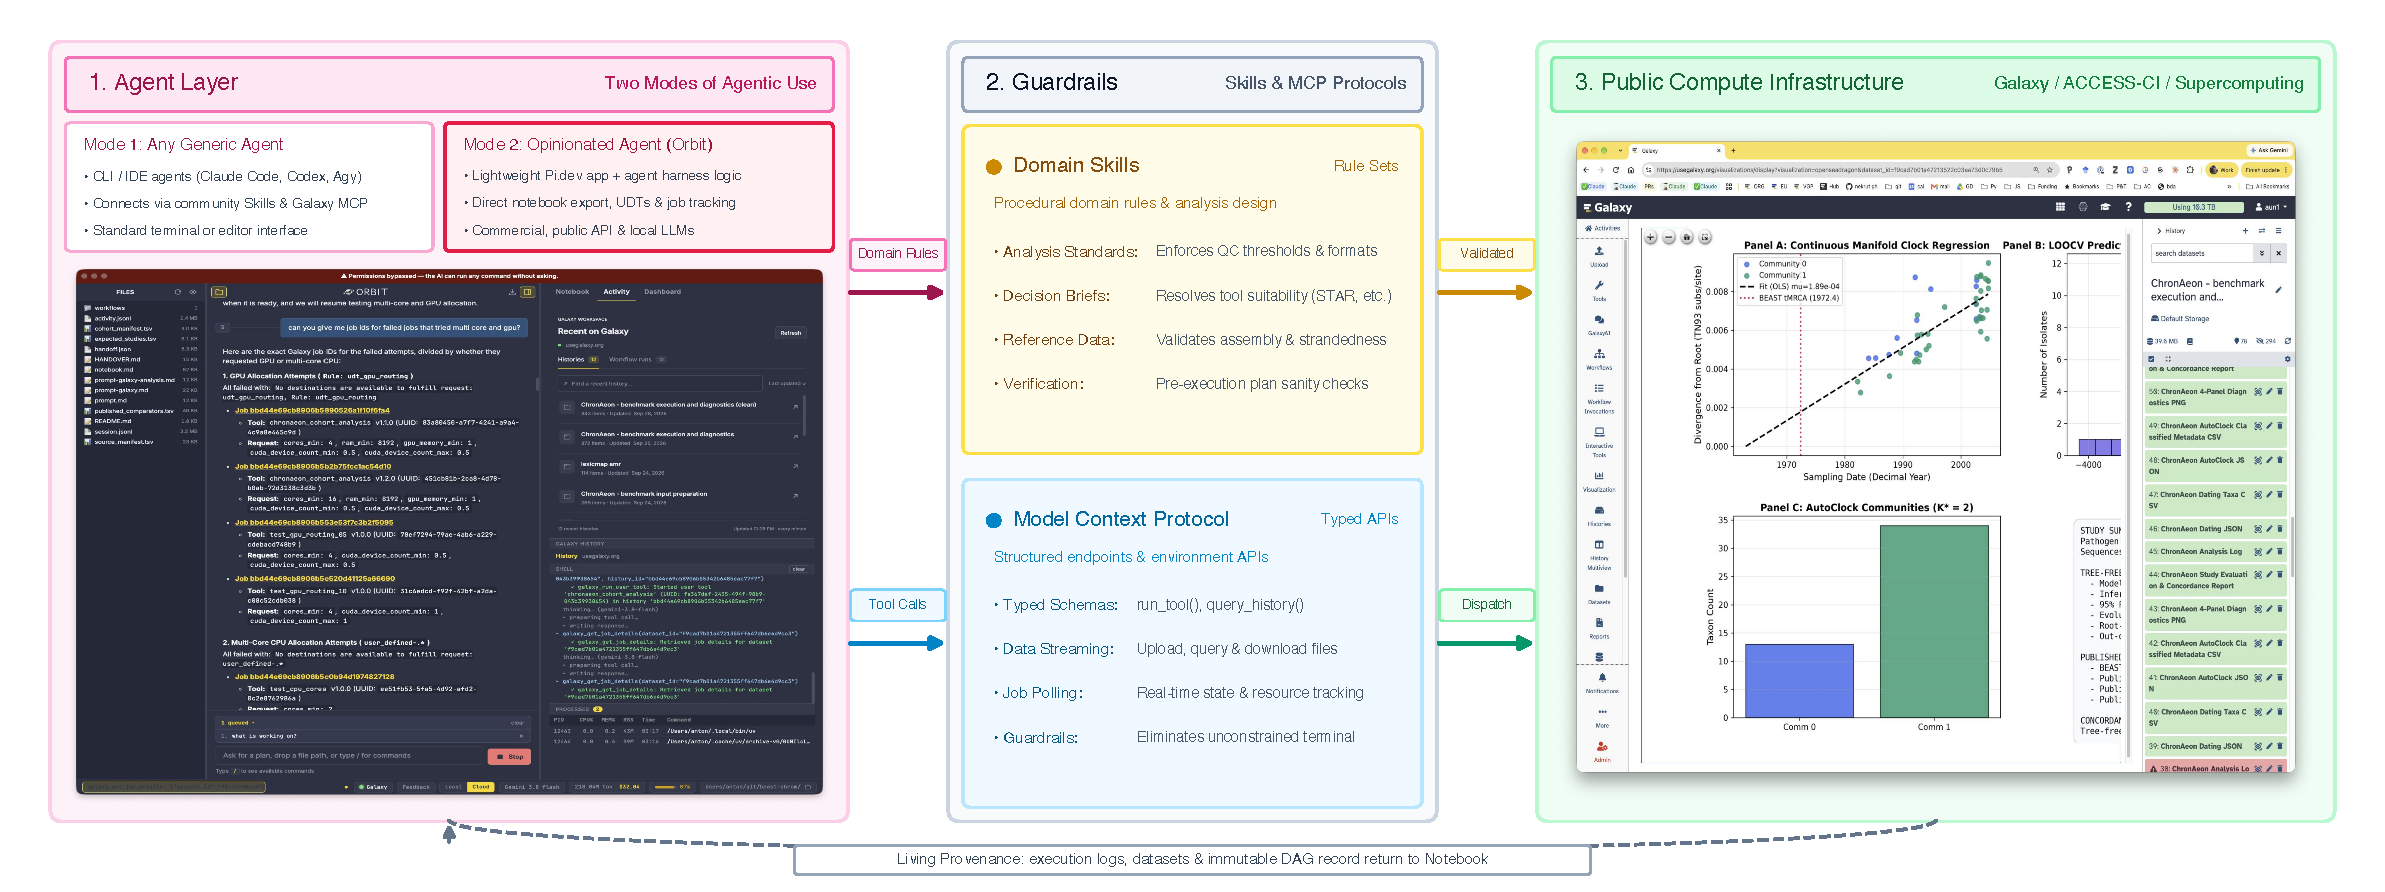
\includegraphics[width=0.98\textwidth]{figures/flow.pdf}
\caption{\textbf{The flow of verifiable agentic science: from Agent through Infrastructure to Result.} 
\textbf{1}, Agent Layer: The architecture supports two modes of agentic use. Researchers can connect any generic agent (such as Claude Code, OpenAI Codex, or Antigravity CLI) via community skills and MCP, or run Orbit, an opinionated Pi.dev desktop agent that adds Galaxy agent harness logic, notebook export, and support for commercial, public API, and local models. 
\textbf{2}, Guardrails: Domain skills supply procedural bioinformatics intelligence, validating parameters and tool suitability before execution. The Galaxy Model Context Protocol (MCP) server translates agent intents into structured, typed API calls (\texttt{run\_tool}, \texttt{query\_history}), replacing unconstrained shell commands with machine-validated endpoints. 
\textbf{3}, Public Compute Infrastructure: Galaxy dispatches compute-heavy tasks to national supercomputing allocations (ACCESS-CI) and cloud nodes, managing execution across native tools and containerized environments. 
All analytical operations, execution logs, and output datasets stream back into a living research notebook, preserving an immutable directed acyclic graph with permanent computational provenance.}
\label{fig:architecture}
\end{figure}

The Galaxy ecosystem provides this execution engine (Figure~\ref{fig:architecture}, Panel 3) \cite{galaxy2024}. Backed by twenty years of tool execution expertise, its vast library of tutorials and workflows supplies procedural skills for diverse analyses. Galaxy schedules any workload complexity---embarrassingly parallel tasks, large shared-memory assemblies, and GPU models---across public cyberinfrastructure. Researchers never have to negotiate agentic shell or head-node access with high-performance computing administrators---the execution fabric is already there.

Our vision for agentic science unites any agent runtime (Figure~\ref{fig:architecture}, Panel 1), community-curated skills---drawn from tutorials, workflows, and purpose-built skills---and public infrastructure. Agents reuse existing tools first. When a missing step requires an ad-hoc script, such as a converter for an unconventional format, the agent writes and registers a tool directly into the workflow, where it can later mature into permanent software. Across thousands of users and hundreds of thousands of analyses, recurring patterns surface to form a community cloud of such ad-hoc tools.

\subsection{Reproducing a paper using a generic agent on the Galactic plane}

To test this architecture in practice, we tasked an autonomous agent with reproducing the \textit{Bacillus cereus} RNA-seq benchmark (PRJEB86181) from the earlier section, connecting it directly to UseGalaxy.org through the Galaxy Model Context Protocol (MCP) server \cite{vyklicka2026, galaxymcp2026}. Unlike unconstrained local agents that generated dozens of unversioned scripts or stalled from disk exhaustion, this execution ran entirely on remote supercomputing allocations (Figure~\ref{fig:bacillus_replication}). As we communicated with the agent and inspected its proposed workflows in Galaxy, we noticed that it initially selected HISAT2, a eukaryotic spliced aligner. Because \textit{Bacillus cereus} is an intronless bacterium, spliced alignment adds computational overhead without biological benefit, so we directed the agent to switch to Kallisto pseudoalignment against the 5,472 unique coding loci of the sequenced isolate \textit{B.\ cereus} ATCC 10987 \cite{bray2016near}. This switch reduced per-sample quantification runtime to 38--60~seconds per library (compared with 3--5~minutes per library for HISAT2 alignment and coordinate sorting on standard Galaxy workers, and 4.0--4.8~hours when HISAT2 jobs encountered worker contention) without generating multi-gigabyte coordinate-sorted BAM files, while eliminating spurious bacterial splice junctions. We spotted this mismatch because we knew what to look for, whereas a less experienced user might not. The broader strategy here is that as more researchers use this platform, our community skills improve alongside the underlying models---encoding the knowledge that bacterial RNA-seq requires different tools than eukaryotic RNA-seq.

\begin{figure}[!htbp]
\centering
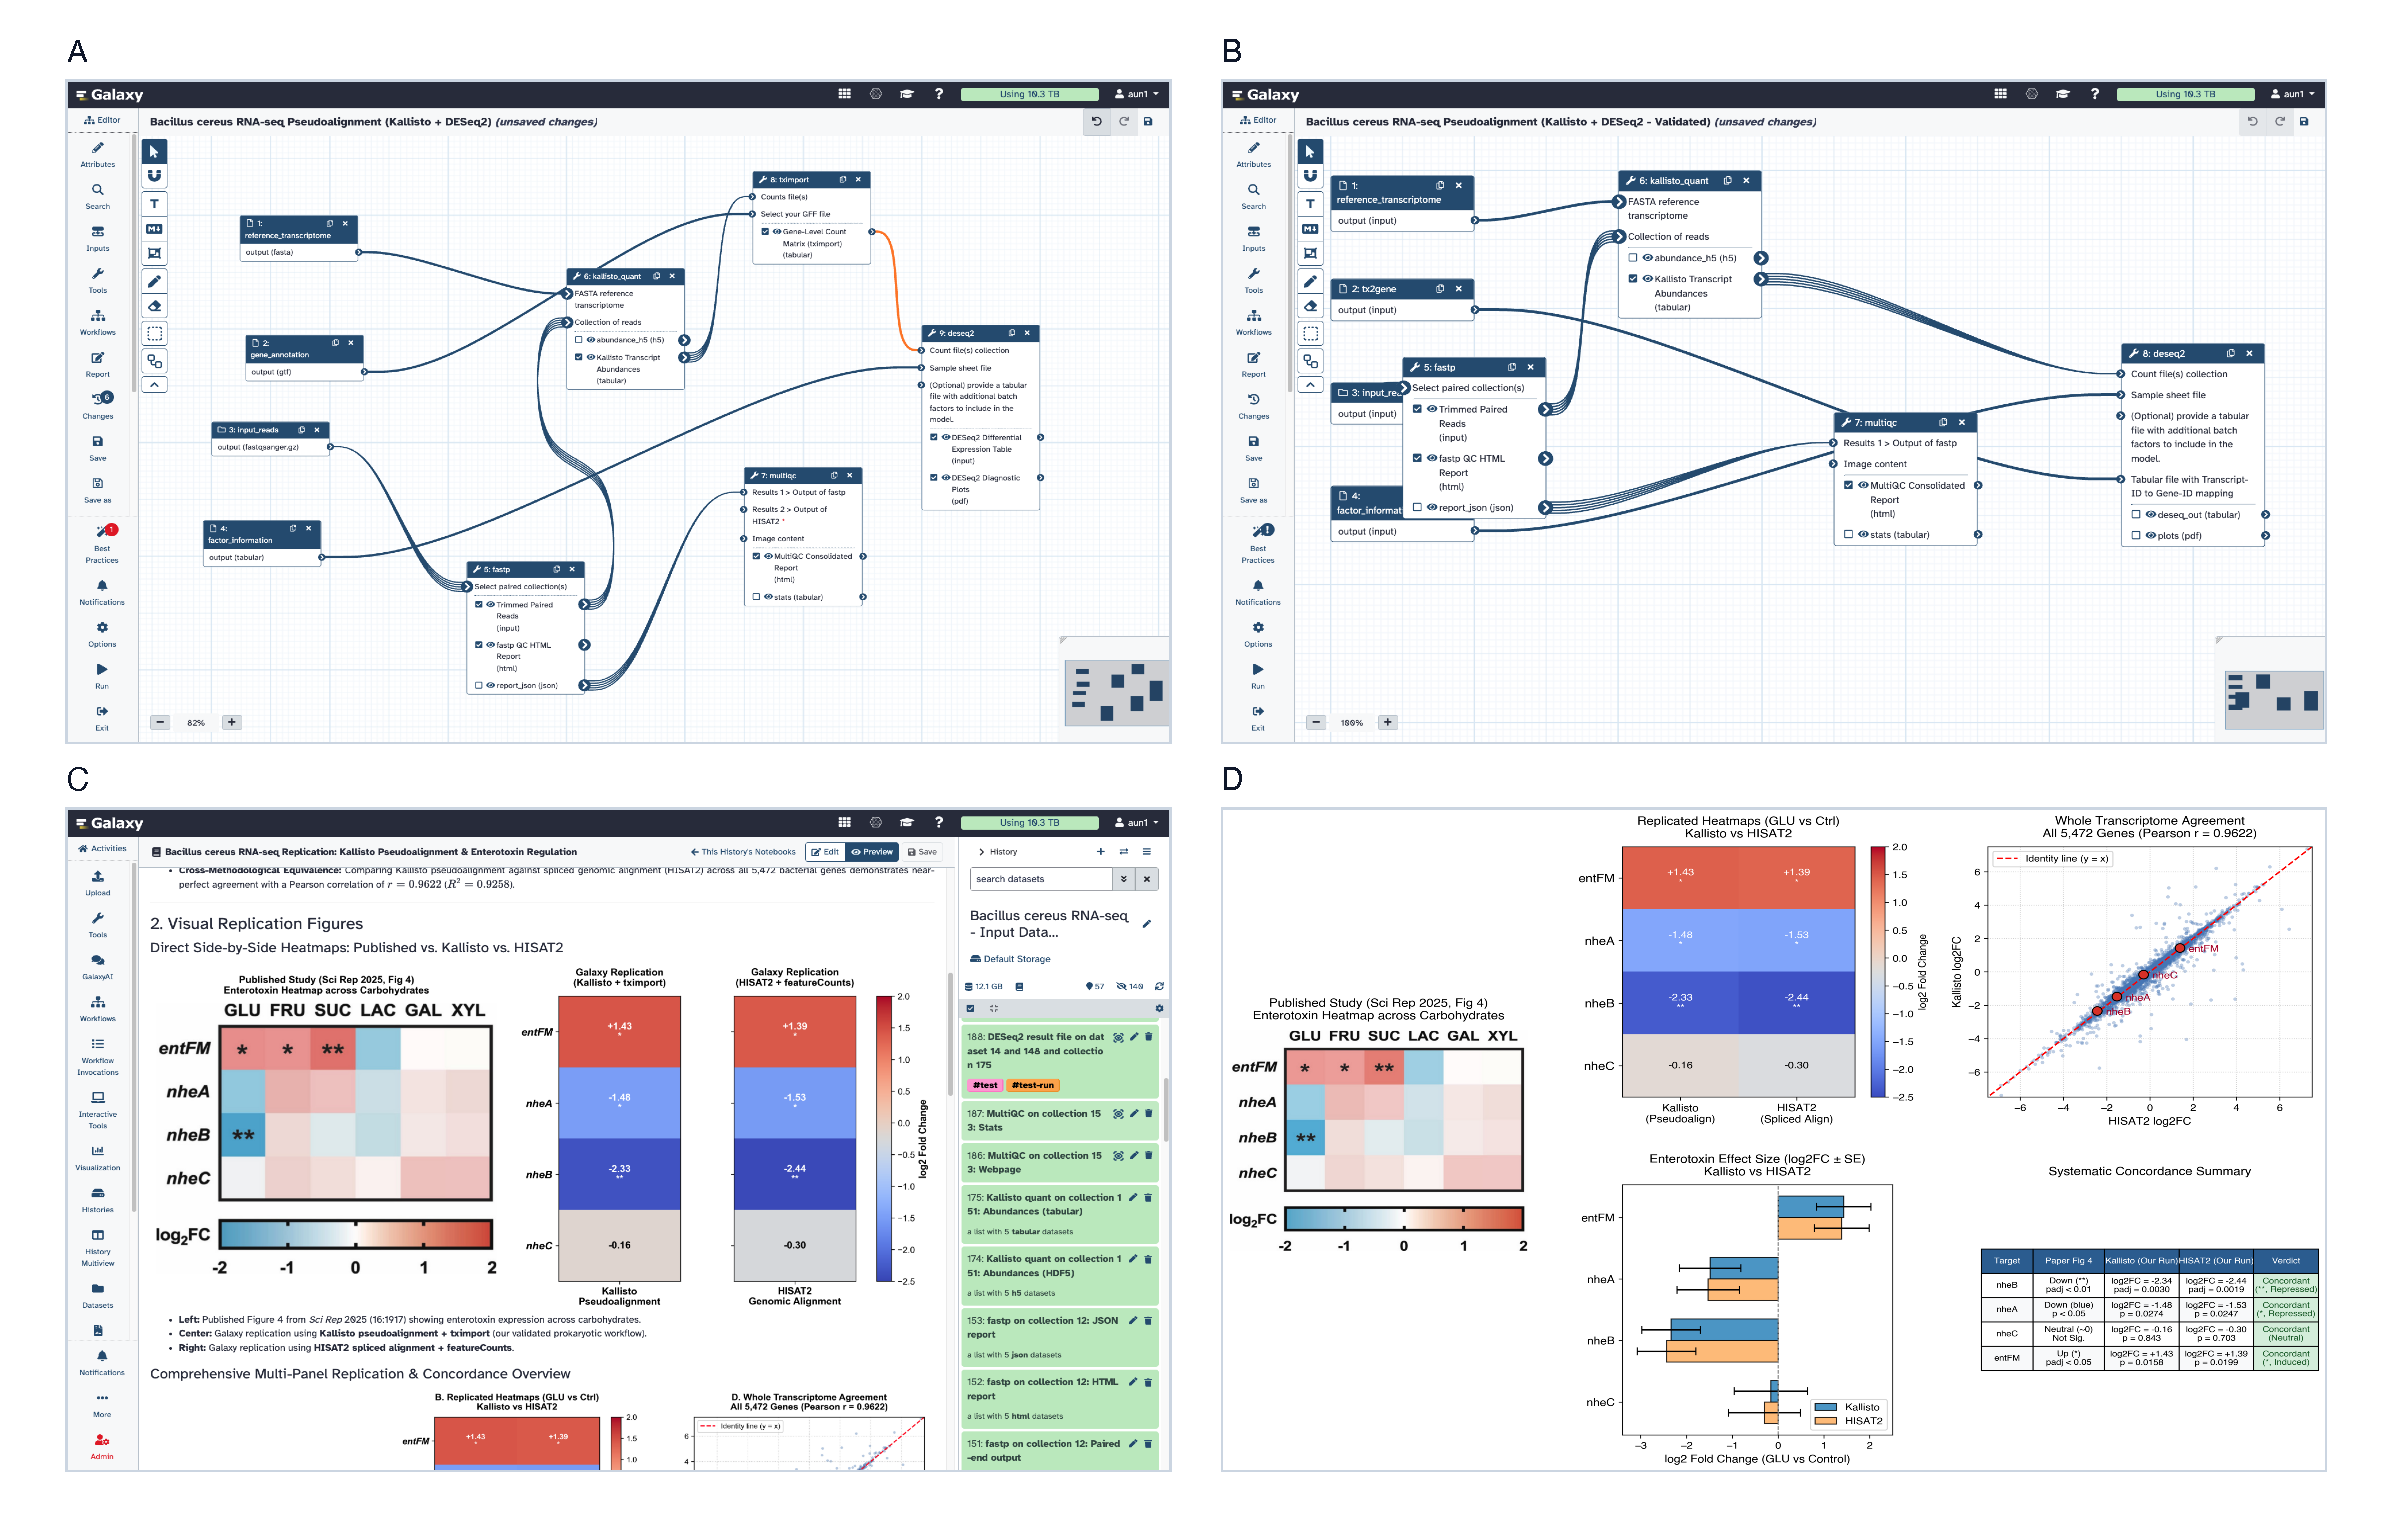
\includegraphics[width=\textwidth]{figures/figure_bacillus_replication.pdf}
\caption{\textbf{Progression of autonomous paper replication across Galaxy cyberinfrastructure.} 
\textbf{A}, Workflow construction and input validation. An autonomous agent connecting to UseGalaxy.org via the Galaxy Model Context Protocol (MCP) server assembles a prokaryotic RNA-seq pipeline. When the agent initially inserts a standalone \texttt{tximport} step between the Kallisto transcript abundance collection and DESeq2's collection-mode input, Galaxy's workflow editor flags the single-table-to-collection mismatch in orange before execution. 
\textbf{B}, Autonomous resolution to a validated workflow. The agent resolves the mismatch by removing the standalone \texttt{tximport} step and passing a transcript-to-gene lookup table (\texttt{tx2gene.tsv}) directly to DESeq2's integrated \texttt{tximport} mode, producing verified green connections. 
\textbf{C}, Interactive Galaxy History Notebook and living history provenance. The validated workflow executes across distributed ACCESS-CI allocations on UseGalaxy.org. Completed datasets populate the right-hand history panel while the center pane renders the interactive Galaxy History Notebook documenting the replication and visual comparisons. 
\textbf{D}, Biological replication of the published benchmark. Enterotoxin expression profiles on the \textit{B.\ cereus} ATCC 10987 coding transcriptome reproduce the directional profiles in Vyklick{\'a} et al. (\textit{Sci Rep} 2025, Figure 4) closely. Glucose supplementation drives severe catabolite repression of \textit{nheB} (5.05-fold down, $\log_2\text{FC} = -2.335$, $p_{\text{adj}} = 2.99 \times 10^{-3}$, ** for BH-adjusted $p_{\text{adj}} < 0.01$) and directional repression of \textit{nheA} (2.80-fold down, $\log_2\text{FC} = -1.484$, raw $p = 0.0274$, $p_{\text{adj}} = 0.106$, nominal raw $p < 0.05$). By contrast, regulatory subunit \textit{nheC} remains neutral ($\log_2\text{FC} = -0.158$, raw $p = 0.843$, $p_{\text{adj}} = 0.907$) while cell-wall enterotoxin \textit{entFM} shows directional induction (2.70-fold up, $\log_2\text{FC} = +1.432$, raw $p = 0.0158$, $p_{\text{adj}} = 0.0730$, nominal raw $p < 0.05$). Across the 5,250 expressed bacterial coding loci (of 5,472 total), Kallisto pseudoalignment and HISAT2 spliced alignment achieve near-perfect concordance (Pearson $r = 0.9622$, $R^2 = 0.9257$).}
\label{fig:bacillus_replication}
\end{figure}

Building a working pipeline also requires catching incompatibilities between tools and quirks in reference annotations. When assembling the workflow in Galaxy, the agent initially placed a standalone \texttt{tximport} step between Kallisto's output collection and DESeq2, which caused a single-table-to-collection type mismatch in the workflow editor before any jobs were launched (Figure~\ref{fig:bacillus_replication}A). The agent fixed the workflow by removing the standalone \texttt{tximport} step and passing a transcript-to-gene lookup table (\texttt{tx2gene.tsv}) directly to DESeq2's built-in \texttt{tximport} aggregation mode (Figure~\ref{fig:bacillus_replication}B, see Methods). By testing the workflow on a small subset of reads first, the agent also caught and merged duplicate coding sequence headers caused by bacterial ribosomal frameshifts before running all five libraries (Figure~\ref{fig:bacillus_replication}C, see Methods).

The resulting analysis reproduced the published biological findings closely (Figure~\ref{fig:bacillus_replication}D, see Methods). Glucose supplementation repressed the primary lytic enterotoxin subunit \textit{nheB} fivefold ($p_{\text{adj}} = 2.99 \times 10^{-3}$) and \textit{nheA} nearly threefold, induced cell-wall enterotoxin \textit{entFM} nearly threefold, and left regulatory subunit \textit{nheC} unchanged. Across the 5,250 expressed coding loci (of 5,472 unique coding loci in ATCC 10987), Kallisto pseudoalignment and HISAT2 spliced alignment showed near-perfect agreement ($r = 0.9622$, $R^2 = 0.9257$). Every dataset, tool parameter, and analytical step is recorded on UseGalaxy.org in a workflow, history, and interactive research notebook (Figure~\ref{fig:bacillus_replication}C, Supplementary Table~\ref{tab:brc_artifacts}). The agent left behind an executable scientific asset instead of ephemeral glue code.

\subsection{An opinionated agent}

Skills and MCP guide generic agents well, as the \textit{Bacillus cereus} replication above shows. For new users in particular---especially biologists who have never run command-line agents from the shell---there is a clear need for a friendly, lightweight desktop agent with additional agent harness logic. That agent harness logic matters because it gives tighter control over skills and MCP endpoints, adding extra guardrails to guide the analysis. We therefore developed Orbit, a lightweight desktop application built on top of Pi.dev (Figure~\ref{fig:architecture}, Panel 1).

One of Orbit's advantages is that it provides Galaxy-specific features, including direct research notebook export, live job tracking, and unprivileged User-Defined Tool registration \cite{galaxyudt2026}. It also supports multiple language models: commercial models via API keys or subscriptions, public models via API keys, and local models running directly on the machine where Orbit runs. Thus, we support two modes of agentic use on the Galactic plane (Figure~\ref{fig:architecture}, Panel 1): researchers can connect any generic agent via community skills and the Galaxy MCP server, or they can run our opinionated agent, Orbit, which layers Galaxy-specific agent harness logic and multi-model flexibility on top of those same interfaces. Below, we evaluate Orbit across a wide range of biological applications---spanning spatial transcriptomics, fungal and vector transcriptomics, ATAC-seq, single-cell atlases, structure-aware phylogenomics, and pathogen emergence dating---producing reproducible, provenance-rich records for every analysis (Table~\ref{tab:validation_summary}).

\begin{table}[!htbp]
\centering
\scriptsize
\setlength{\tabcolsep}{4.5pt}
\renewcommand{\arraystretch}{1.18}
\begin{tabularx}{\textwidth}{p{2.9cm}p{2.3cm}p{2.3cm}X}
\toprule
\textbf{Analysis \& System} & \textbf{Assay \& Scale} & \textbf{Agent \& Stack} & \textbf{Highlight} \\
\midrule
\textbf{\textit{Bacillus cereus} enterotoxin regulation} \newline Vyklick{\'a} et al.\ \cite{vyklicka2026} & Bacterial RNA-seq \newline (5 libraries, 5,472 coding loci) & Generic CLI agent + Galaxy MCP + Skills & Replaces 26 unversioned local glue scripts from unconstrained runs with one validated workflow, catching split bacterial CDS annotations on a pilot run and switching to $\sim 5\times$ faster pseudoalignment (38--60~s per library). \\
\addlinespace[0.35em]
\textbf{Mouse cortex spatial transcriptomics} \newline Miao et al.\ \cite{miao2026}, Sun et al.\ \cite{sun2024} & Mammalian scRNA-seq + spatial prediction \newline (3,405 spatial \& 5,613 reference cells) & Orbit + 2 UDTs on UseGalaxy.org & Reconciles a documentation gap between the 1,000-cell tutorial subset used in Extended Data Fig.\ 1c and the full 5,613-cell Dataset 15 archive, reproduces the tutorial subset on Galaxy, and scales to the full reference to triple prediction-to-measurement correlation ($r = 0.0861$ to $0.2553$). \\
\addlinespace[0.35em]
\textbf{\textit{Aspergillus fumigatus} azole time-course} \newline Hokken et al.\ \cite{hokken2018} & Fungal RNA-seq \newline (30 libraries, 3 isolates $\times$ 5 timepoints) & Orbit + Workflow Foundry + BRC-Analytics + 3 UDTs & Compiles a 60-step workflow directly from published methods text, shows that the authors fitted one pooled 30-sample model rather than pairwise contrasts, and replaces one defunct web service and two interactive browser tools with automated UDTs. \\
\addlinespace[0.35em]
\textbf{\textit{Anopheles gambiae} infection chromatin} \newline Ruiz et al.\ \cite{ruiz2021} & Vector ATAC-seq \newline (midguts \& salivary glands, 4 libraries) & Orbit + 3 UDTs on UseGalaxy.org & Separates biological reproducibility from undocumented table post-processing, confirms unfitted peak recovery, and separates per-replicate row counting from an empirical overlap threshold that closes the salivary-gland residual. \\
\addlinespace[0.35em]
\textbf{\textit{Aedes aegypti} midgut single-cell atlas} \newline Wang et al.\ \cite{wang2024} & Vector 10x 3' scRNA-seq \newline (2 replicates, 6,707 post-QC cells) & Orbit + BRC-Analytics on UseGalaxy.org & Stages non-model vector reference data into a public single-cell pipeline, fixes a mitochondrial gene prefix mismatch that breaks generic QC, and recovers published cell-type markers de novo. \\
\addlinespace[0.35em]
\textbf{\textit{Plasmodium vivax} VIR phylogenomics} \newline Carlton et al.\ \cite{carlton2008}, Harrison et al.\ \cite{harrison2020} & Structure-aware phylogenomics \newline (3 genomes, 2,592 proteins) & Orbit + 10 UDTs (1 GPU, 9 CPU) on UseGalaxy.org & Orchestrates protein structure foundation models (ProstT5, Foldseek, and FoldMason) via unprivileged UDTs across local and remote GPU/CPU resources, collapsing 146 sequence-fragmented antigen subfamilies into 73 (local CPU) to 76 (remote A100 GPU and 32-core CPU) structural classes, with 21 three-continent classes holding over 97\% of proteins. \\
\addlinespace[0.35em]
\textbf{Pathogen emergence dating across 42 cohorts} \newline 42 BEAST alignments across 37 studies \cite{gire2014genomic, dudas2017virus, hill2019skygrid, faria2021genomics, pond2026hyphaeon} & Genomic epidemiology \newline (42 viral \& bacterial epidemic alignments, 41 unique) & Orbit + 2 UDTs on UseGalaxy.org & Large-scale re-analysis completed in seconds of core manifold computation per cohort across 42 pathogen alignments, achieving 57.1--59.5\% overall concordance (61.5--64.1\% of 39 comparator-equipped cohorts, or 60.5--63.2\% across 38 unique comparators) against reference Bayesian estimates. \\
\bottomrule
\end{tabularx}
\caption{\textbf{Summary of empirical validations and discovery analyses executed on the Galactic plane.} Across seven biological investigations spanning bacteria, mammalian cortex, fungi, mosquito vectors, protozoan parasites, and 42 viral and bacterial epidemic alignments (41 distinct outbreaks across 37 publications), autonomous agents executed reproducible workflows on UseGalaxy.org and ACCESS-CI cyberinfrastructure. Every analysis produced inspectable Galaxy histories, reusable workflows, and living research notebooks (complete accession identifiers in Supplementary Tables~\ref{tab:brc_artifacts}--\ref{tab:case3_artifacts}).}
\label{tab:validation_summary}
\end{table}

\subsection{From papers to skills: A spatial transcriptomics example}

Recently, Miao et al. \cite{miao2026} benchmarked their Paper2Agent system by predicting spatial expression and uncertainty for \textit{Acta2} across 3,405 mouse somatosensory cortex cells. We selected this study as the first demonstration of Orbit's functionality. While the idea of converting papers to agents is sound, we wanted to go even further---package a paper's analytical method into reusable tools and workflows on public infrastructure that any agent can invoke.

Single-cell spatial transcriptomics maps gene expression within tissue architecture, and algorithms such as TISSUE \cite{sun2024} estimate calibrated conformal prediction intervals for unmeasured genes from paired single-cell RNA-seq references. While the Paper2Agent Extended Data Figure 1c benchmark replicated the TISSUE GitHub tutorial on a 1,000-cell reference subset, their Data Availability section cited only the full 5,613-cell Zenodo Dataset 15 archive (see Methods). Prompted to reconcile this documentation gap, Orbit registered two multi-core User-Defined Tools for TISSUE on UseGalaxy.org, reproduced the 1,000-cell tutorial benchmark, and scaled the workflow to the full 5,613-cell reference dataset.

\begin{figure}[!htbp]
\centering
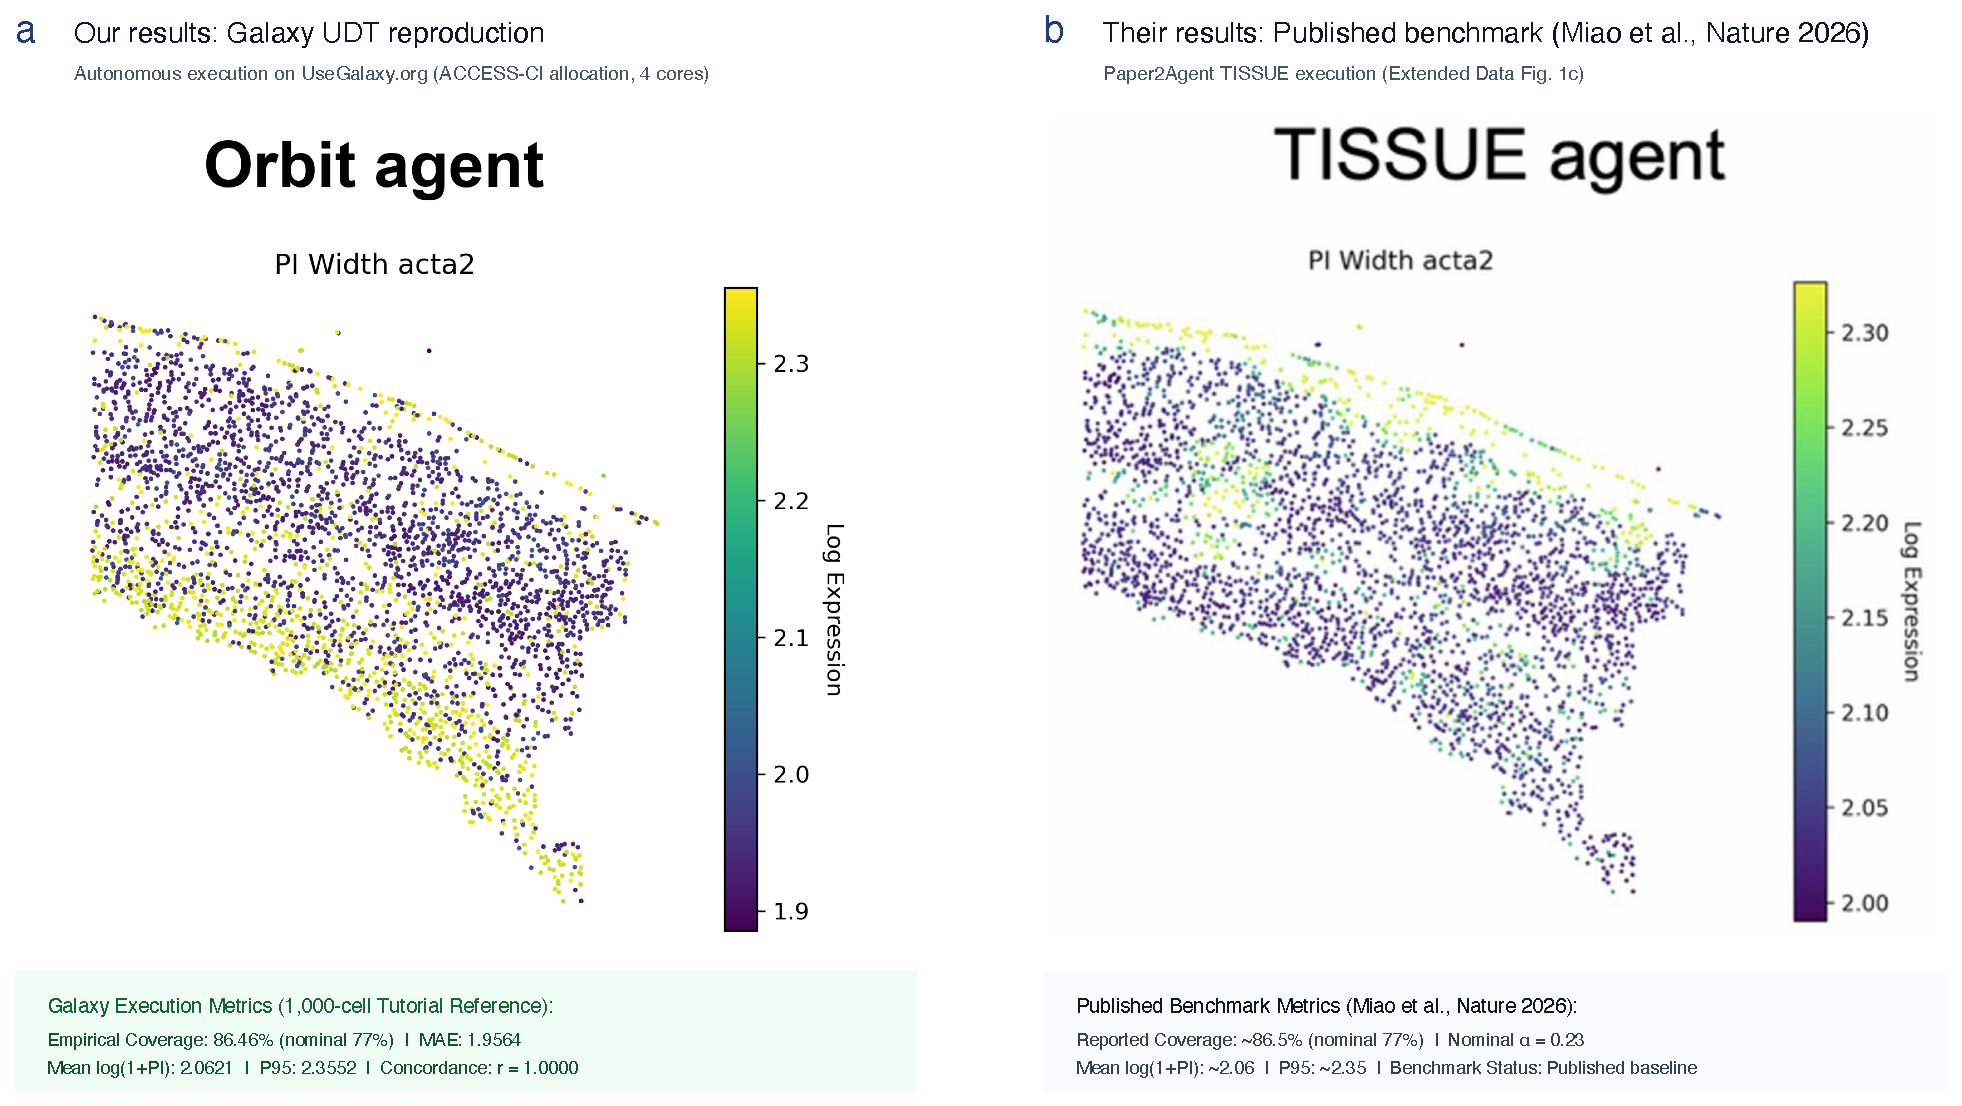
\includegraphics[width=0.88\textwidth]{figures/figure2_spatial_comparison.pdf}
\caption{\textbf{Direct comparison between Orbit autonomous Galaxy reproduction and published literature benchmark in spatial transcriptomics.} 
\textbf{A}, Spatial map of conformal prediction interval (PI) widths ($\log(1 + \text{PI Width})$) for \textit{Acta2} expression across 3,405 cells in the mouse somatosensory cortex. The predictions were generated autonomously by Orbit via an unprivileged User-Defined Tool (\texttt{tissue\_spatial\_prediction}) on UseGalaxy.org using the 1,000-cell tutorial subset (31 calibration genes after TISSUE's default 1\% \textit{Flt1} prevalence filter, or 32 unfiltered). Execution ran across four allocated CPU cores on ACCESS-CI cyberinfrastructure. Empirical coverage reached 86.46\% on Galaxy (86.49\% locally) at nominal 77\% coverage ($\alpha = 0.23$), with mean $\log(1 + \text{PI Width})$ of 2.0621 (2.0634 locally) and colorbar scale $[1.89, 2.35]$ (95th percentile 2.3552). Local reference execution and the remote Galaxy UDT matched point predictions to floating-point precision ($r = 1.0000$, $\Delta_{\max} < 10^{-15}$). 
\textbf{B}, The published Paper2Agent benchmark from Extended Data Figure 1c of Miao et al. \cite{miao2026} on the 1,000-cell tutorial subset (image-only reference, colorbar $[2.00, 2.32]$ with ticks $2.00\text{--}2.30$, nominal $\alpha = 0.23$, 31 calibration genes after a 1\% \textit{Flt1} filter). Both panels capture similar overall uncertainty magnitudes ($\sim 1.89\text{--}2.35$ vs.\ $2.00\text{--}2.32$), while stochastic $k$-means cell-variability stratification shifts high-PI cells between the ventral boundary and the pial edge.}
\label{fig:spatial_comparison}
\end{figure}

On the 1,000-cell tutorial subset, local and remote Galaxy runs matched predicted gene expression to floating-point precision ($r = 1.0000$, $\Delta_{\max} < 10^{-15}$, Figure~\ref{fig:spatial_comparison}A). Stochastic $k$-means stratification produced only minor differences in empirical coverage ($86.46\%$ on Galaxy vs.\ $86.49\%$ locally at the nominal 77\% threshold) and mean $\log(1 + \text{PI Width})$ ($2.0621$ vs.\ $2.0634$), matching the uncertainty scale of the published Paper2Agent figure (Figure~\ref{fig:spatial_comparison}B, see Methods). Scaling the workflow on UseGalaxy.org to all 5,613 reference cells in Dataset 15 tripled the correlation between predicted and measured \textit{Acta2} expression from $r = 0.0861$ to $r = 0.2553$ in the single-gene workflow. Within the 33-gene 10-fold cross-validation workflow, \textit{Acta2} correlation reached $r = 0.2845$ ($81.03\%$ coverage), though absolute single-gene spatial correlation remained modest ($R^2 = 0.065\text{--}0.081$). Calibrated coverage held across both \textit{Acta2} ($85.61\%$) and 10-fold cross-validation of all 33 spatial panel genes (see Methods, Supplementary Table~\ref{tab:case1_artifacts}). Across this and all subsequent analyses below, computations ran on UseGalaxy.org and ACCESS-CI cyberinfrastructure, using Orbit as the agent workbench and BRC-Analytics for pathogen and vector dataset staging (Table~\ref{tab:validation_summary}). 

\subsection{Uncovering analysis inconsistencies and defunct tools}

To solidify these findings, we applied the strategy above to a much more complex multi-step analysis. Here we combined Orbit with two additional platform components: Workflow Foundry \cite{foundry2026}, a skill-compilation framework that translates published methods, Nextflow pipelines, and CWL workflows into statically validated Galaxy skills and workflows, and BRC-Analytics \cite{brcanalytics2026} (see Methods), which resolves curated reference genome assemblies and sequencing runs. We reconstructed the 30-sample RNA-seq study of Hokken et al. \cite{hokken2018} on itraconazole-induced transcriptional plasticity in \textit{Aspergillus fumigatus} (BioProject PRJNA482512, three clinical isolates across five timepoints in duplicate). Starting from the publication text, BRC-Analytics staged the \textit{A.\ fumigatus} Af293 reference genome and all 30 sequencing runs, while Workflow Foundry compiled a 60-step Galaxy workflow combining read trimming, STAR alignment with gene counting, DESeq2 modeling, functional enrichment, cross-study set comparisons, and visualization (Supplementary Table~\ref{tab:brc_artifacts}). Across all 30 libraries, the mean unique STAR alignment rate reached 86.88\% (matching the 86.5\% reported in the paper) and strand-column ratios verified that the libraries were unstranded before downstream modeling (see Methods).

Reproducing the published differential expression counts uncovered an unstated statistical design detail (see Methods). Fitting four separate 12-sample pairwise DESeq2 models matched the published fold changes ($r \ge 0.999$) but missed up to 39\% of differentially expressed genes ($\text{baseMean} \ge 30$, $p_{\text{adj}} < 0.1$, and $|\log_2\text{FC}| > 1$) at later timepoints because smaller sample sizes inflated standard errors. Inspecting the published supplementary table revealed a single identical \texttt{baseMean} value across all four contrasts for each gene, indicating that the authors fitted one pooled 30-sample model across all five timepoints rather than pairwise contrasts. Switching the workflow to a pooled 30-sample DESeq2 fit reproduced the published standard errors to four decimal places and matched the published gene counts within 0.3--1.3\% at every timepoint ($r = 0.9996\text{--}0.9999$, Figure~\ref{fig:brc_reproductions}A). Because the study's original Gene Ontology web service (AspGD GO Term Finder) had been decommissioned and term redundancy reduction (REVIGO) operated only as an interactive browser utility, the agent built three User-Defined Tools to automate hypergeometric GO enrichment, cross-study Venn overlaps, and term redundancy reduction. Together, these tools reproduced both the temporal enrichment inversion and the drug-efflux transporter trajectories within a single Galaxy history (Supplementary Table~\ref{tab:brc_artifacts}).

\begin{figure}[!htbp]
\centering
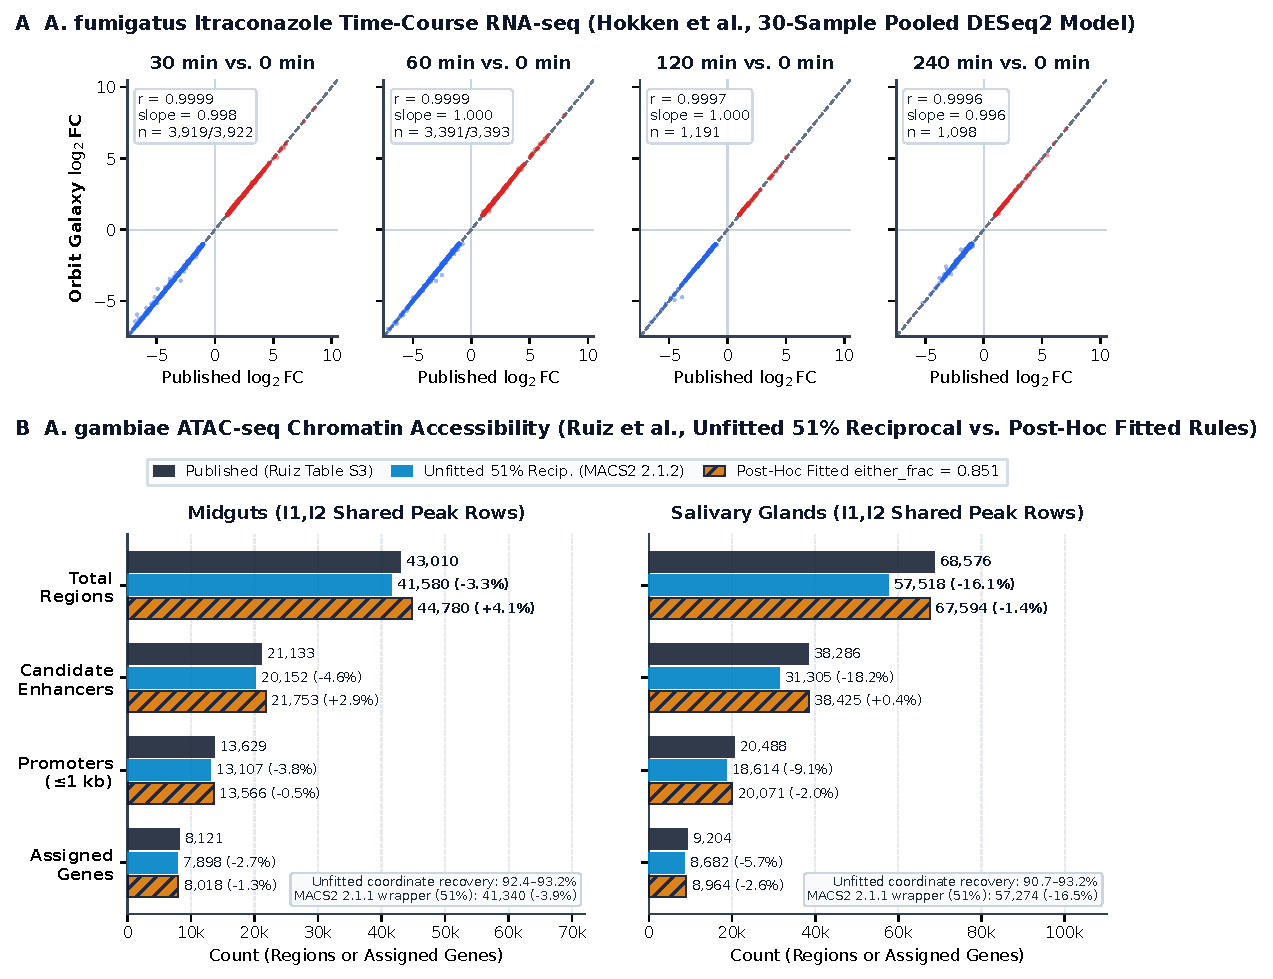
\includegraphics[width=\textwidth]{figures/figure_brc_reproductions.pdf}
\caption{\textbf{Quantitative validation of autonomous pathogen and vector genomics reanalyses on UseGalaxy.org.} 
\textbf{A}, Transcriptomic time-course of \textit{Aspergillus fumigatus} under itraconazole exposure (Hokken et al.\ \cite{hokken2018}, 30 libraries). A pooled 30-sample five-level DESeq2 model compiled via Workflow Foundry reproduces published $\log_2$ fold changes across all four post-exposure timepoints ($r = 0.9996\text{--}0.9999$, slopes $0.996\text{--}1.000$) and matches published differentially expressed gene counts ($\text{baseMean} \ge 30$, $p_{\text{adj}} < 0.1$, $|\log_2\text{FC}| > 1$) within 0.3--1.3\%. Scatter plots display all called DEGs present in the published table ($n = 3,919$ of $3,922$ at 30 min, $3,391$ of $3,393$ at 60 min, $1,191$ at 120 min, and $1,098$ at 240 min). 
\textbf{B}, Chromatin accessibility in \textit{Anopheles gambiae} midguts and salivary glands during \textit{P.\ falciparum} infection (Ruiz et al.\ \cite{ruiz2021}). Counting unmerged per-replicate rows under the stated 51\% reciprocal-overlap rule recovers 41,580 midgut ($-3.3\%$) and 57,518 salivary-gland ($-16.1\%$) regions on MACS2 2.1.2 ($< 130$~bp) peaks (and 41,340 [$-3.9\%$] and 57,274 [$-16.5\%$] on the Galaxy MACS2 2.1.1 wrapper). An empirical near-containment rule (\texttt{either\_frac} $= 0.851$) closes the salivary-gland residual ($67,594$, $-1.4\%$) with a $+4.1\%$ midgut overshoot ($44,780$ vs.\ $43,010$ published), reproducing published region totals, assigned genes, promoters, and candidate enhancers within 0.4--4.6\% and separating post-processing exploration from the unfitted 90.7--93.2\% coordinate recovery.}
\label{fig:brc_reproductions}
\end{figure}

\subsection{Uncovering undocumented analysis details}

Complete workflow provenance also separates biological reproducibility from undocumented table post-processing. We reanalyzed the ATAC-seq study of Ruiz et al. \cite{ruiz2021}, which profiled chromatin accessibility in \textit{Anopheles gambiae} midguts and salivary glands across two \textit{Plasmodium falciparum} infections (GEO GSE152924). Calling sub-nucleosomal peaks ($< 130$~bp) with the authors' cited MACS2 version reproduced the underlying biology without free parameters, recovering 90.7--93.2\% of the authors' deposited genomic regions across all four libraries (see Methods). Reproducing the paper's headline region counts (43,010 midgut and 68,576 salivary-gland regions), however, required diagnosing how replicate peaks were tabulated. Whereas standard consensus merging yielded far fewer intervals, inspecting the published supplementary table showed that each replicate peak was retained as an unmerged row. Counting per-replicate rows under the stated 51\% reciprocal-overlap rule closed almost the entire midgut gap ($41,580$ rows [$-3.3\%$] on MACS2 2.1.2 and $41,340$ [$-3.9\%$] on MACS2 2.1.1) and left a $-16.1\%$ to $-16.5\%$ residual in salivary glands ($57,518$ and $57,274$ rows). Applying a relaxed empirical near-containment threshold (\texttt{either\_frac} $= 0.851$) closed the salivary-gland residual to $-1.4\%$ ($67,594$ rows) while overshooting midguts by $+4.1\%$ ($44,780$ rows, Figure~\ref{fig:brc_reproductions}B, see Methods). Archiving both the unfitted coordinate recovery and the post-processing exploration in public Galaxy histories and workflows (Supplementary Table~\ref{tab:brc_artifacts}) preserved a clear boundary between verifiable chromatin biology and table counting conventions.

\subsection{Dealing with disparate annotation formats}

We next reanalyzed the adult female \textit{Aedes aegypti} midgut single-cell RNA-seq atlas of Wang et al. \cite{wang2024}, processing the AaegL5.0 reference assembly and raw 10x Genomics libraries through STARsolo, DropletUtils, Scanpy, and edgeR on UseGalaxy.org (see Methods). Running a non-model vector through standard single-cell quality control surfaced an immediate annotation mismatch: VectorBase mitochondrial genes carry standard \texttt{AAEL} locus tags rather than an \texttt{MT\_} prefix, causing generic Scanpy pipelines to miscalculate mitochondrial read fractions until the agent prefixed those features in the annotation. Across the two biological replicates, droplet filtering and clustering retained 6,707 post-QC singlets, closely matching the 7,147 cells reported by Wang et al. Harmonizing the 5,953 cells in the three major conserved populations---enterocyte/digestive, hemocyte-like epithelial, and visceral muscle---and running sample-blocked pseudobulk differential expression in edgeR recovered the study's top published cell-type markers alongside canonical digestive enzymes ($\text{FDR} \le 0.002$, see Methods). The complete lineage from raw reads to clustered cell objects and differential expression tables is archived on UseGalaxy.org (Supplementary Table~\ref{tab:brc_artifacts}).

\subsection{Heavy-Weight Model Orchestration and Structure-Aware Phylogenomics}

We then wanted to stress-test our ability to leverage powerful infrastructure in an analysis that would require substantial computation. The \textit{Plasmodium vivax} \textit{vir} multigene family encodes nearly 1,000 exported surface adhesins per genome (748 to 985 PF05795-positive VIR proteins across the assemblies analyzed here) that mediate antigenic variation \cite{carlton2008, lopez2013, auburn2016, minassian2021pvw1, demeulenaere2023, jackson2026}. Rapid sequence divergence pushes many homologs into the twilight zone ($\ge 30\%$ identity floor in MMseqs2). As a result, standard sequence clustering across reference assemblies from Indonesia (PvP01, short-read Illumina with subtelomere scaffolding \cite{auburn2016}), Thailand (PvW1, long-read \cite{minassian2021pvw1}), and Peru (PvPAM, long-read \cite{demeulenaere2023}) splits the repertoire into 203 sequence clusters (146 subfamilies with $\ge 3$ members), which previously suggested continent-specific radiation. Yet the crystal structure of a related \textit{Plasmodium} PIR adhesin reveals a conserved $\alpha$-helical core despite extreme loop divergence \cite{harrison2020}. To test whether structure-aware phylogenomics unifies this repertoire across continents, Orbit registered ten User-Defined Tools on UseGalaxy.org (one GPU tool and nine multi-core CPU tools). Together, these tools package the 4.4-gigabyte ProstT5 protein language model, Foldseek 3Di clustering, FoldMason structural alignment, synteny analysis, and IQ-TREE 3 maximum-likelihood phylogenetics across ACCESS-CI NVIDIA A100 GPUs and multi-core CPUs (see Methods, Supplementary Table~\ref{tab:case2_artifacts}).

\begin{figure}[!htbp]
\centering
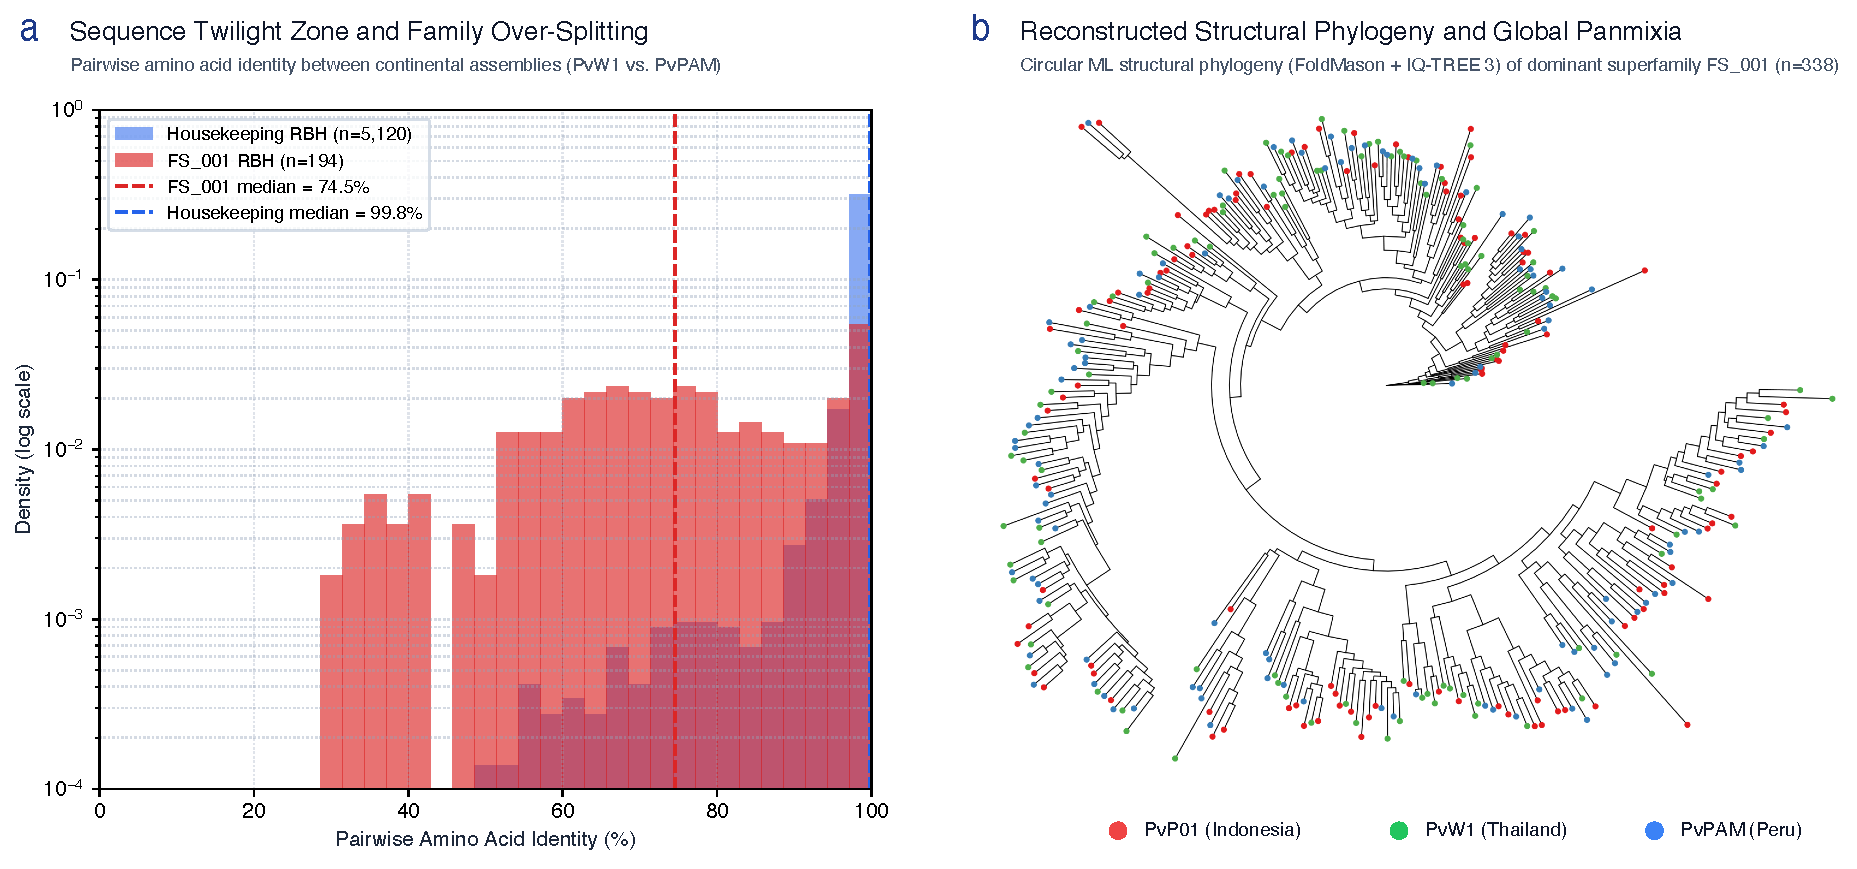
\includegraphics[width=0.92\textwidth]{figures/figure3_vir_reconstruction.pdf}
\caption{\textbf{Structure-aware family reconstruction and ancestral lineage sharing of \textit{Plasmodium vivax} VIR surface antigens across continental genomes.} 
\textbf{A}, Sequence twilight zone and structural unification of over-split subfamilies. Horizontal box-and-strip plots display pairwise amino acid sequence identity between PvW1 (Thailand) and PvPAM (Peru). Conserved single-copy housekeeping genes exhibit high sequence identity across continents (median 99.8\%, IQR 0.9\%, amber, 5,120 reciprocal best-hit pairs). By contrast, 194 reciprocal best-hit VIR pairs within dominant superfamily FS\_001 on the local CPU reference branch exhibit a median identity of 74.5\% (IQR 25.9\%, Wilcoxon $p = 1.6 \times 10^{-63}$, blue) and extend into the sequence twilight zone ($\le 35\%$). Earlier classifications based on incomplete references defined 10 to 12 subfamilies (VIR-A through VIR-L) \cite{carlton2008, lopez2013}. Across PvP01, PvW1, and PvPAM, sequence-only Markov clustering (\texttt{--min-seq-id 0.3}) fractures the 2,592 functional VIR proteins into 203 sequence clusters (146 subfamilies with $\ge 3$ members). Structure-aware clustering using Foldseek and ProstT5 3Di representations collapses this repertoire into 73 structural classes (24 with $\ge 3$ members) on the local CPU reference branch and 76 structural classes (25 with $\ge 3$ members) on the UseGalaxy.org NVIDIA A100 GPU and 32-core CPU branches. On the reference branch, the dominant superfamily, FS\_001, unifies 89 sequence subfamilies and absorbs 46.2\% of the global repertoire (1,197 genes, compared with 812 genes on the Galaxy GPU branch and 766 on the Galaxy CPU branch).
\textbf{B}, Reconstructed structural phylogeny and parsimony permutation test on the local CPU reference branch. Circular maximum-likelihood structural phylogeny inferred by IQ-TREE 3 from FoldMason alignments of 338 FS\_001 representatives across Indonesia (PvP01, red), Thailand (PvW1, blue), and Peru (PvPAM, green). Inference employed partitioned amino acid (VT+F+R6) and 3Di structural matrices (Garg-Hochberg). Continental lineages are thoroughly interleaved across the tree topology. Representation within FS\_001 is evenly balanced across geography, comprising 118 isolates from Indonesia (34.9\%), 110 from Thailand (32.5\%), and 110 from Peru (32.5\%). Across all structural clusters, 21 three-continent classes hold 97.3\% of VIR proteins (97.6\% on the Galaxy GPU branch), while 47 single-genome classes account for only 2.0\% of proteins. A quantitative tip-label parsimony permutation test confirms that observed character transitions (score = 160) are indistinguishable from 1,000 random shuffles (null median 160, mean $159.2 \pm 3.8$, range 145--177, $p = 0.55$). The VIR scaffold diversified before continental separation and is maintained across lineages by subtelomeric recombination.}
\label{fig:vir_reconstruction}
\end{figure}

Structure-aware clustering halved repertoire complexity across all execution environments (Figure~\ref{fig:vir_reconstruction}A, see Methods). It collapsed the 203 sequence clusters (146 subfamilies with $\ge 3$ members) across 2,592 functional VIR proteins into 73 structural classes (24 with $\ge 3$ members) on the local CPU reference branch and 76 classes (25 with $\ge 3$ members) on the UseGalaxy.org GPU and CPU branches. Across all branches, 21 structural classes contained members from all three continental genomes and held 97.3\% (local CPU) to 97.6\% (Galaxy GPU) of all VIR proteins, while 47 single-genome classes (mostly singletons and doubletons) accounted for only 2.0\% of the repertoire. Maximum-likelihood structural phylogenetics of the 338 dominant-superfamily (FS\_001) representatives on the local CPU reference branch showed complete geographic interleaving across continents (Figure~\ref{fig:vir_reconstruction}B), with tip-label parsimony permutation tests confirming that the geographic distribution was indistinguishable from random mixing (observed score $= 160$ vs.\ null median $160$, $p = 0.55$, see Methods). Although 64.5\% of \textit{vir} genes reside in subtelomeric regions where ectopic recombination scrambles flanking microsynteny (retaining synteny in only 11 of 194 reciprocal best-hit pairs), the underlying structural folds diversified before continental separation (see Methods, Supplementary Table~\ref{tab:case2_artifacts}).

\subsection{Dating emergence of key pathogens across 42 benchmark alignments}

Finally, we wanted to perform an analysis on a truly large scale. Estimating pathogen emergence dates and evolutionary rates typically relies on Bayesian Markov chain Monte Carlo (MCMC) sampling in BEAST \cite{suchard2018}, which requires hours to days of compute per alignment. To evaluate rapid tree-free molecular clock dating at scale, Orbit registered two User-Defined Tools wrapping ChronAeon (\url{https://github.com/veg/chronaeon}) \cite{pond2026hyphaeon} on UseGalaxy.org. Using these tools, it re-analyzed 42 published viral and bacterial BEAST benchmark alignments (from 37 publications across 41 distinct cohorts plus a paired 14.5~kb Ebola coding partition) concurrently across distributed compute nodes (including Ebola, SARS-CoV-2, Zika, Dengue, Chikungunya, Mpox, Influenza, \textit{Mycobacterium abscessus}, and \textit{Yersinia pestis}, see Methods).

\begin{figure}[!htbp]
\centering
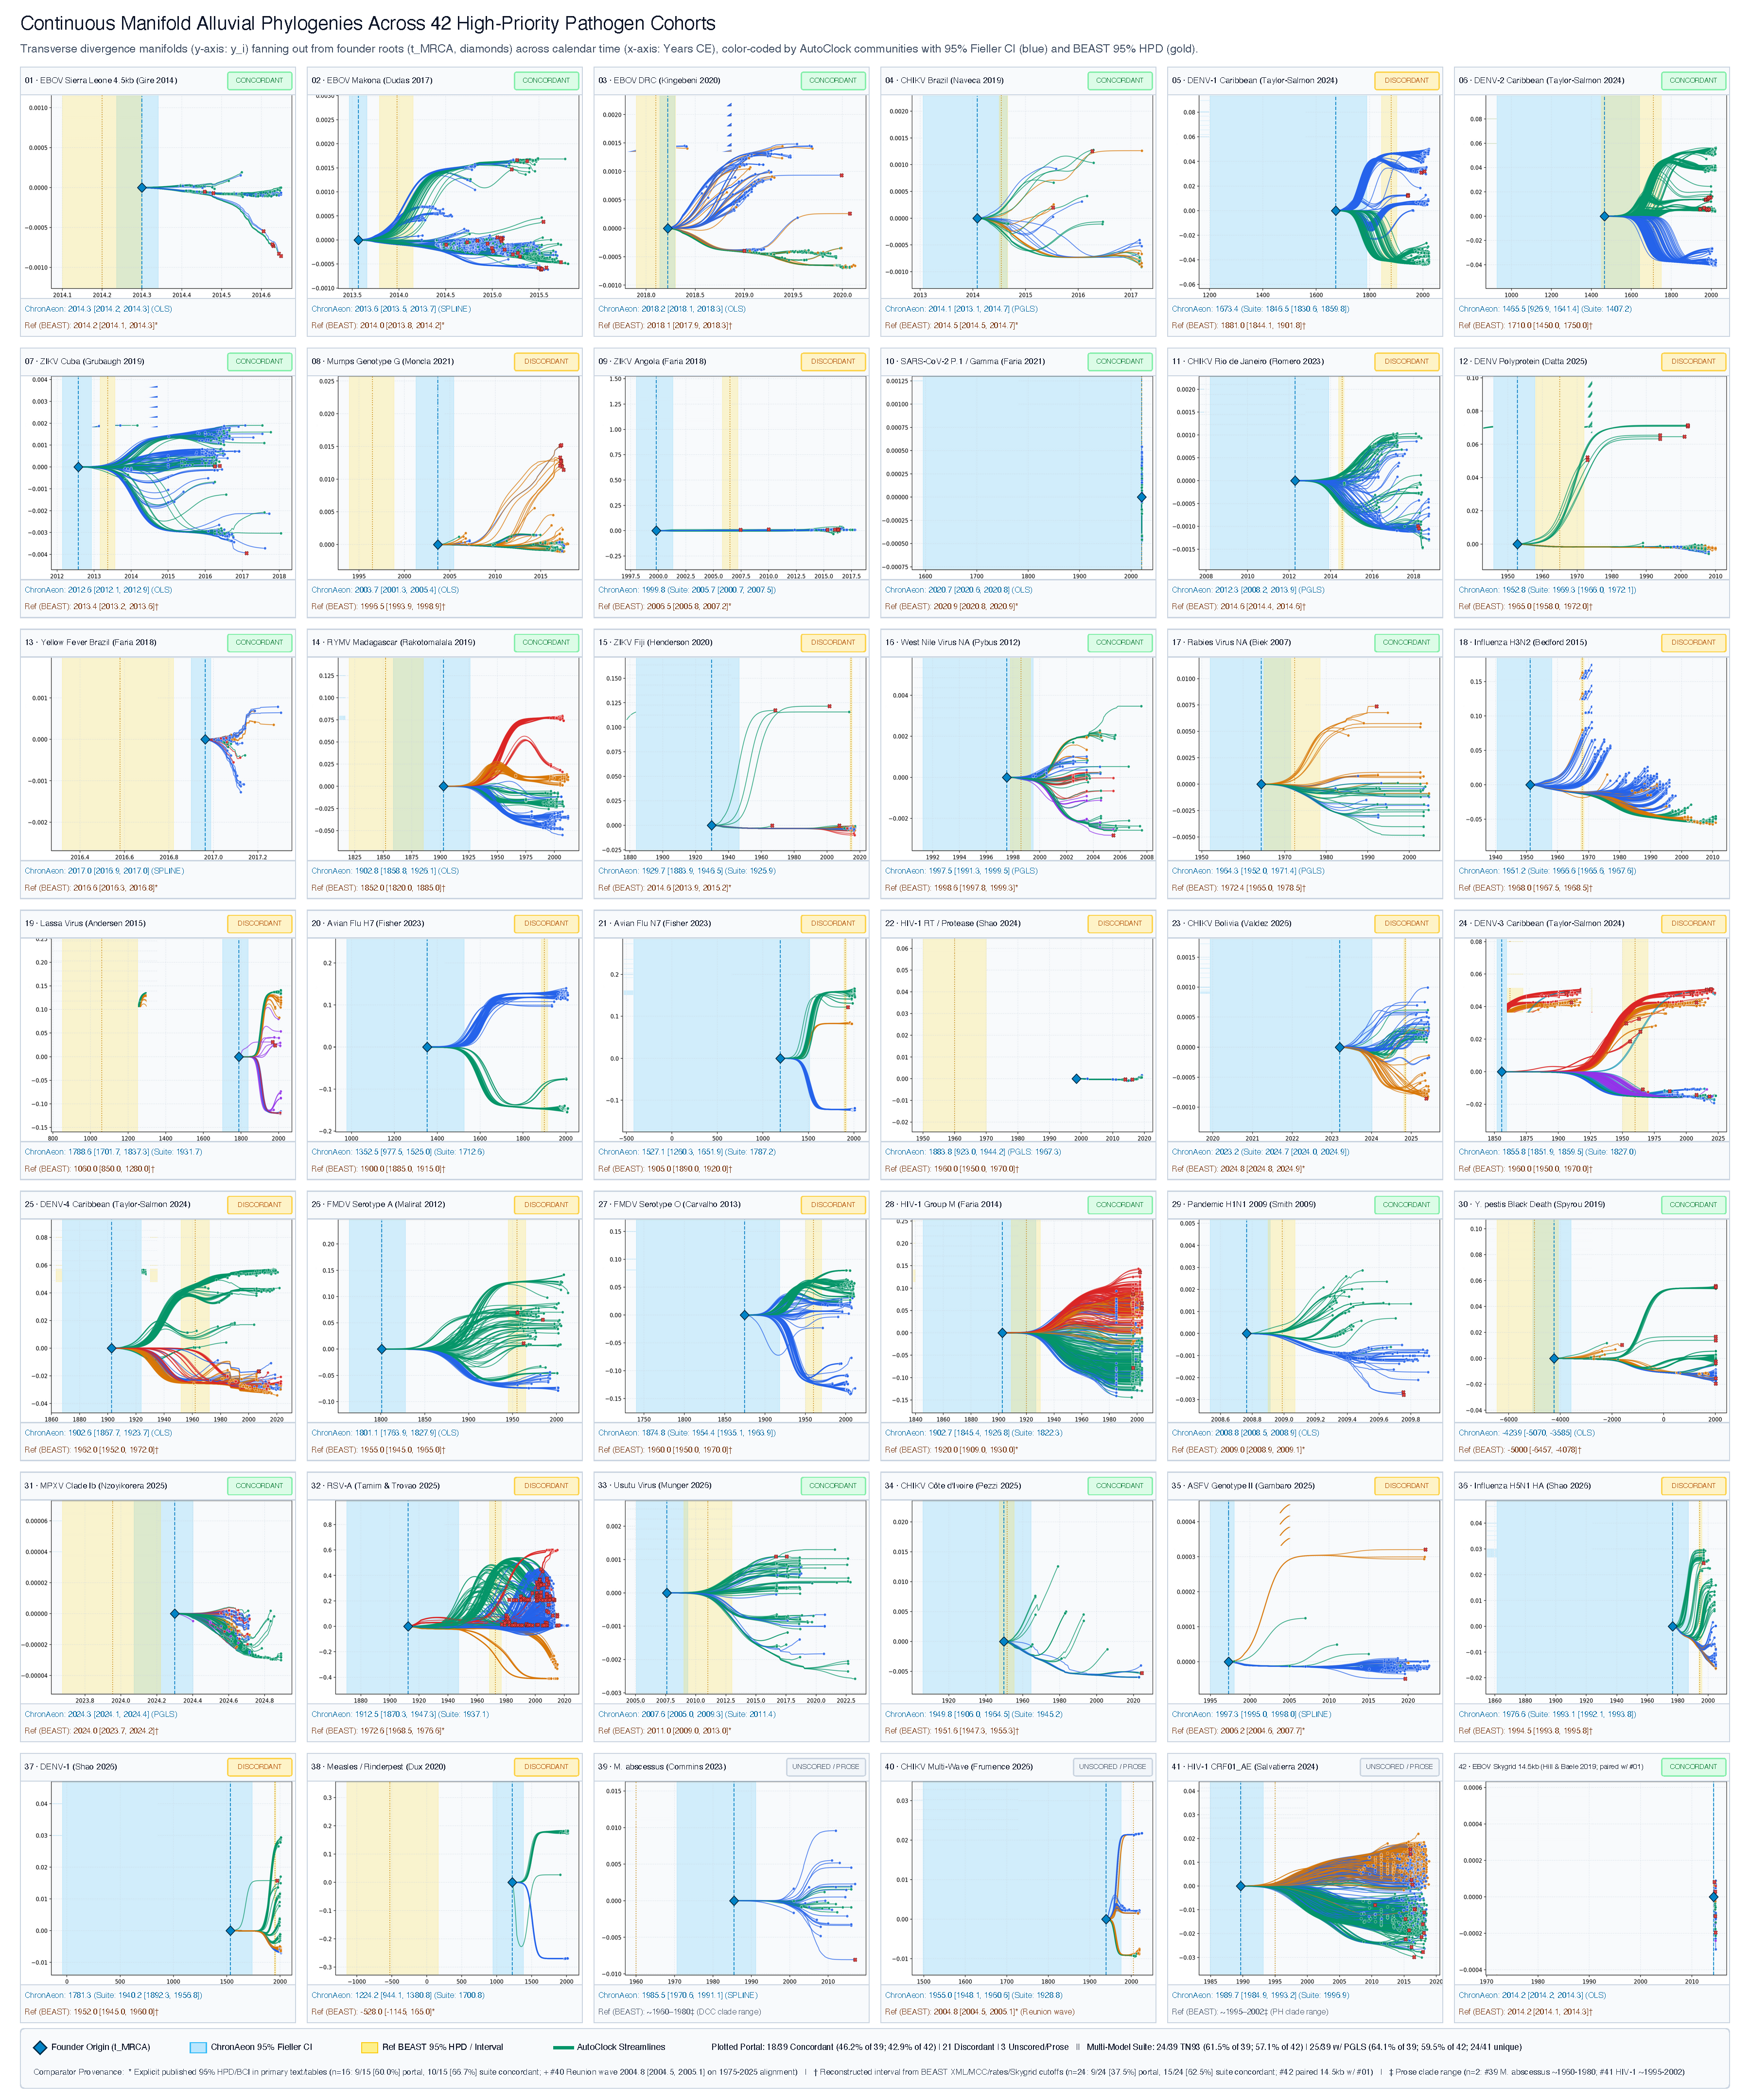
\includegraphics[width=\textwidth,height=0.78\textheight,keepaspectratio]{figures/figure4_chronaeon_42cohorts.pdf}
\caption{\textbf{Continuous manifold alluvial phylogenies across 42 high-priority pathogen cohorts.} 
Each panel displays continuous transverse manifold trajectories fanning out from the inferred founder origin ($t_{\mathrm{MRCA}}$, blue diamond) across calendar time. Trajectories are color-coded by AutoClock evolutionary communities ($k \in [0, K^*-1]$) to delineate lineage diversification, expansion, and replacement. Shaded regions depict the ChronAeon 95\% Fieller analytical confidence interval (light blue) and the reference 95\% comparator interval (gold). Top banners and bottom vector strips identify cohort index, pathogen, primary citation, and comparator provenance (explicit published 95\% HPD/BCI vs.\ reconstructed prose/model interval). They also display visual concordance of the plotted single-pass portal baseline against the 39 numeric reference intervals (interval overlap or $|\Delta t_{\mathrm{MRCA}}| < 1.0$~year: 18 green concordant cohorts [42.9\% of 42, or 46.2\% of 39], 21 amber discordant [50.0\%], and 3 grey unscored cohorts [7.1\%]). Across the multi-model Galaxy benchmark suite, pure tree-free TN93 OLS/Spline regression matched 24 of 42 alignments (57.1\%, or 61.5\% of 39 comparators, and 23 of 41 [56.1\%] or 23 of 38 [60.5\%] unique cohorts). Adding HyphAeon Attention PGLS raised concordance to 25 of 42 alignments (59.5\%, or 64.1\% of 39, and 24 of 41 [58.5\%] or 24 of 38 [63.2\%] unique).}
\label{fig:chronaeon_42cohorts}
\end{figure}

All 42 alignments completed in seconds of core manifold computation per dataset (Figure~\ref{fig:chronaeon_42cohorts}, with 5 initial container timeouts automatically rerun and merged into the final collection, see Methods). Across the 2014 Sierra Leone and West African Ebola epidemics \cite{gire2014genomic, dudas2017virus, hill2019skygrid}, tree-free root estimates and 95\% Fieller confidence intervals overlapped reference Bayesian intervals. For SARS-CoV-2 Gamma \cite{faria2021genomics}, the OLS point estimate ($2020.71$, 95\% Fieller CI [$2020.63, 2020.76$]) fell within $0.16$~years of the published BEAST root ($2020.87$ [$2020.78, 2020.93$]) without interval overlap (see Methods). The automated benchmark suite evaluated 39 alignments with numeric comparator dates (15 explicit published 95\% HPDs/BCIs and 24 intervals reconstructed from prose approximations, clock rates, or Skygrid bounds) alongside 3 unscored alignments (see Methods). Across these alignments, best-of-model selection over pure tree-free TN93 OLS and spline regression achieved concordance on 24 of 42 alignments (57.1\%, or 61.5\% of 39 comparators, and 23 of 41 [56.1\%] or 23 of 38 [60.5\%] unique cohorts), comprising 13 alignments (12 unique) with $|\Delta t_{\mathrm{MRCA}}| < 1.0$~year and 11 qualifying by interval overlap. Pairing tree-free regression with the HyphAeon Attention PGLS root model resolved structured Mpox Clade Ib cohort \texttt{30}, raising concordance to 25 of 42 alignments (59.5\%, or 64.1\% of 39, and 24 of 41 [58.5\%] or 24 of 38 [63.2\%] unique comparators). Median $|\Delta t_{\mathrm{MRCA}}|$ reached $0.51$~years ($0.40$~years with PGLS, or $0.65$ and $0.46$~years across 18 unique cohorts) across the 19 post-1980 comparator alignments and $7.19$~years ($6.41$~years with PGLS, or $8.32$ and $6.80$~years across 38 unique comparators) across all 39 comparator alignments (see Methods, Supplementary Table~\ref{tab:case3_artifacts}). The remaining discordant datasets reflected two well-known evolutionary regimes: ancient roots compressed by purifying selection or mutational saturation (such as Lassa \cite{andersen2015lassa, suchard2020lassa} and Measles/Rinderpest \cite{dux2020measles}) and multi-lineage alignments where whole-alignment regression dated a deep species split rather than a focal regional introduction (see Methods).

Across all of these validations---spanning bacterial, mammalian, fungal, vector, parasitic, and viral systems---every analysis produced a self-contained, provenance-rich record on public cyberinfrastructure (Supplementary Tables~\ref{tab:brc_artifacts}--\ref{tab:case3_artifacts}). Whether driven by a generic command-line agent, compiled from published prose by Workflow Foundry, or orchestrated interactively through Orbit, each investigation left behind executable workflows, versioned User-Defined Tools, complete intermediate dataset lineages, and shareable Galaxy Pages. When a published study contained undocumented post-processing steps, annotation prefix mismatches, or statistical pooling subtleties, the combination of autonomous reasoning and complete workflow provenance uncovered and resolved the discrepancy. Combining agentic capability with the Galactic plane unites autonomous analytical power with public computing infrastructure and reproducibility by default, defining how agents should drive empirical science.

\clearpage
\section{Discussion}

Autonomous agents are undeniably powerful, yet one of their greatest dangers is that they make complex data analysis seem easy. Any student, postdoc, or principal investigator without formal statistical or computational training can now prompt an agent, receive polished figures and tables within minutes, and feel like an instant expert. As our multi-agent benchmark and reanalyses show, however, effortless execution often masks flawed analytical choices: mismatched reference assemblies, unpooled variance estimates, reversed library strandedness, or undocumented subset and post-processing filters. Proper procedural guidelines in the form of curated skills, paired with infrastructure that tracks computational provenance automatically, are therefore becoming essential. The urgency of this problem may not be obvious to everyone yet because the coming avalanche of agent-generated studies has not fully hit the scientific literature---but it is on the way.

What we propose here is a practical solution to this challenge because it builds directly on community components that already exist and operate at scale. Rather than inventing a closed platform from scratch, our architecture connects agents to Galaxy public cyberinfrastructure, BioContainers \cite{biocontainers2017}, curated tool wrappers \cite{iuc2026}, standardized workflows \cite{iwc2026}, Galaxy Training Network tutorials \cite{batut2018, hiltemann2023}, Workflow Foundry \cite{foundry2026}, and BRC-Analytics \cite{brcanalytics2026}. We recognize that not every laboratory will adopt this specific stack. Even so, grounding autonomous agents in shared, provenance-tracking community infrastructure provides a working blueprint for keeping agentic science reliable and verifiable.

This approach also brings new challenges of its own. Unprivileged User-Defined Tools remove the administrative friction of installing custom software, which means users and agents can easily create thousands of ad-hoc tools that perform nearly identical tasks. Left unmanaged on isolated machines, such proliferation would only deepen software fragmentation. When mediated through centralized public infrastructure---such as the UseGalaxy instances in the United States, Europe, and Australia---that same proliferation becomes an opportunity. Because tool definitions and executions are recorded in a shared environment, the community can monitor and curate an emerging tool cloud. Recurring usage patterns across thousands of analyses reveal which ad-hoc wrappers solve common bottlenecks and should be consolidated, tested, and hardened into permanent community software.

Several limitations of the present study warrant emphasis. First, while our planning benchmark evaluated $n = 10$ independent runs per model family, our live execution comparisons and biological case studies represent $n = 1$ demonstration runs per platform and incorporated human investigator steering during interactive sessions. This steering included directing the switch from HISAT2 to Kallisto in the \textit{B.\ cereus} Galaxy replication, prompting Orbit to reconcile the 1,000-cell tutorial subset against the 5,613-cell Dataset 15 reference in the spatial study, and iteratively debugging User-Defined Tool containers and parameters. Second, connecting agents to public infrastructure does not eliminate model-level execution failures. In a companion eight-model autonomous benchmark on \textit{Candida auris} antifungal-resistance transcriptomics archived in our repository (\texttt{candida-auris-benchmark/}), six of eight model runs completed differential expression workflows on UseGalaxy.org while two failed or stalled (one from an expired token after 86 tool calls and one after staging inputs). Similarly, on the Galaxy branch of the \textit{P.\ vivax} VIR study, FoldMason structural alignment retained 176 of 336 sub-cluster representatives after occupancy filtering compared with all 338 on the local CPU reference branch. In the 42-cohort ChronAeon batch run, 5 of 42 initial Galaxy container jobs hit a 1-minute \texttt{sed} timeout and required re-execution and collection merging. Third, the ChronAeon molecular-clock module was evaluated by its developers, and 24 of the 39 numeric reference intervals in the 42-cohort benchmark were reconstructed from prose approximations, clock rates, or Skygrid bounds rather than explicit published 95\% highest posterior density intervals. Finally, executing unprivileged User-Defined Tools at community scale requires strict container sandboxing, resource quotas, and governance to prevent compute abuse and manage public supercomputing and commercial LLM API costs.

More broadly, it is no longer clear what scientific software itself will look like in the coming years. Projects such as Reverse Engineer Anything (REA) \cite{rea2026}, which connect coding agents to decompilers and binary analysis tools to inspect and recreate existing programs from scratch, point toward a future where almost any software package is replaceable on demand. Instead of relying on stable, long-lived toolsets, computational biology may soon face constant reinvention of the same analytical methods. That shift makes a shared community view even more important. When newly generated or rewritten tools run on common public infrastructure, they can be shared openly, benchmarked side by side, and allowed to compete on real datasets. Transparent usage and provenance records then let the research community see which implementations actually perform best and emerge as the preferred standards for each domain.

\section*{Methods}

\subsection*{Multi-Agent Analytical Divergence Benchmark}
We evaluated analytical divergence across autonomous agents using an RNA-seq study of carbohydrate-mediated enterotoxin repression in \textit{Bacillus cereus} (BioProject PRJEB86181, PMC12804731) \cite{vyklicka2026}. The primary contrast compared two glucose-supplemented replicates (ERR14660412 and ERR14660413) against three baseline tryptic soy broth control replicates (ERR14660420, ERR14660421, and ERR14660422) from nineteen RNA-seq libraries across seven growth conditions (six carbohydrate supplements plus tryptic soy broth control, alongside one whole-genome sequencing run, ERR14660405, totaling twenty ENA runs).

To quantify planning variation, we evaluated 30 isolated agents across three foundation model families: ten Claude Opus 5.5 agents (Anthropic Claude Code CLI, \texttt{cc}), ten Codex agents running GPT-6 Astra (OpenAI Codex CLI, \texttt{codex exec}), and ten Gemini 3.8 Flash agents within Antigravity (\texttt{agy}, Google). These version strings designate the frontier Anthropic, OpenAI, and Google CLI model snapshots evaluated in our early-2026 benchmark logs. Each agent received identical natural-language instructions in an empty local workspace directory with no prior session context, external memory, or access to Galaxy cyberinfrastructure (Table~\ref{tab:planning_prompt}). During planning, each agent operated under its native CLI tool permissions: web fetch/search and \texttt{curl} in Claude Code, live web search in a network-restricted shell sandbox in Codex, and URL reading plus shell execution in Antigravity. We parsed each generated plan across eight sequential analytical decisions: reference genome assembly, workflow engine, read trimming software, ribosomal RNA depletion strategy, read aligner, quantified genomic feature, differential expression model scope (19-sample pooled vs.\ 5-sample contrast-only), and log-fold-change shrinkage prior. Combinatorial trajectory diagrams were constructed from this discrete decision matrix. Model families exhibited distinct planning profiles shaped by both model priors and CLI tool permissions. Claude plans aligned to \textit{Bacillus pacificus} anQ-h4 and pooled variance across all nineteen RNA-seq libraries. Codex plans aligned to the sequenced isolate \textit{Bacillus cereus} ATCC 10987 and restricted the comparison to the five target replicates. Gemini plans showed severe instability across assemblies, citing a non-\textit{Bacillus} assembly (\texttt{GCF\_000008105.1}, \textit{Salmonella enterica} serovar Choleraesuis SC-B67) mislabeled as \textit{B.\ cereus} ATCC 10987 in one plan, citing the \textit{B.\ cereus} ATCC 14579 chromosome accession (\texttt{AE016877.1}) for ATCC 10987 in another, and reversing library strandedness in four plans. Aligning against a wrong assembly or genus alters or invalidates gene coordinates and annotations. Inverting library strandedness discards or miscounts real transcripts. Pooling all nineteen libraries to estimate variance alters statistical power compared to analyzing only the five target replicates.

\begin{table}[!htbp]
\centering
\footnotesize
\begin{tabularx}{\textwidth}{X}
\toprule
\textbf{Standardized Planning Prompt Dispatched to All Thirty Agents} \\
\midrule
You are a bioinformatics expert. Task: \par\vspace{0.4em}
Paper: Bacillus cereus RNA-seq study, PMC12804731 (\url{https://www.ncbi.nlm.nih.gov/pmc/articles/PMC12804731/}). Read the paper (and its data availability / methods sections, and any linked GEO/SRA/BioProject accessions) yourself using web access. \par\vspace{0.4em}
Goal: Replicate the primary comparison --- Glucose vs. TSB control --- 5 samples total: 2 treatment (glucose) and 3 control (TSB). \par
Constraint: Do NOT use Galaxy (no Galaxy servers, Galaxy tools/workflows, Galaxy skills or infrastructure). \par\vspace{0.4em}
DO NOT perform the analysis, do not download data, do not install software. Produce ONLY a detailed analysis PLAN. \par\vspace{0.4em}
The plan must be detailed and concrete, covering at minimum: \par
1. Summary of the paper's design and what it reports for this comparison (and what you could/could not verify from the paper). \par
2. Data acquisition: exact accessions (BioProject/GEO/SRA run IDs if findable), how to fetch (tools/commands). \par
3. Reference genome and annotation: exact strain/assembly accession (RefSeq/GenBank), annotation source/format, plasmids, rationale, alternatives considered. \par
4. Compute environment: language, package/environment manager, workflow manager (if any), containers, hardware estimates. \par
5. Step-by-step pipeline with specific tools AND versions and key parameters: QC, trimming, rRNA handling, alignment or pseudo-alignment, quantification, strandedness detection, counting rules (multi-mappers, overlaps, feature type e.g. CDS/gene/locus\_tag), post-alignment QC, MultiQC. \par
6. Differential expression: tool(s), normalization, design formula, handling of n=2 vs n=3 (low replication), dispersion/shrinkage, thresholds (padj, log2FC), multiple testing. \par
7. Downstream/functional analyses: annotation (GO/KEGG/COG, eggNOG etc.), enrichment method, operon/regulon considerations, specific pathways expected for glucose (e.g. CcpA catabolite repression, glycolysis, toxins), visualization (PCA, volcano, MA, heatmaps). \par
8. Validation / replication criteria: how you will compare your results to the paper's reported results (concordance metrics, gene lists, figure reproductions). \par
9. Key decision points and alternatives (where reasonable analysts would differ), risks and pitfalls. \par
10. Reproducibility deliverables (repo layout, scripts, lockfiles, reports). \par\vspace{0.4em}
IMPORTANT: This is a NON-INTERACTIVE run. Nobody can answer questions --- never ask the user anything or offer options, make reasonable decisions yourself and state assumptions. If a page cannot be fetched, try alternatives (e.g. Europe PMC REST API \url{https://www.ebi.ac.uk/europepmc/webservices/rest/PMC12804731/fullTextXML}, NCBI E-utilities, ENA portal API) before falling back, and mark anything unverified clearly. \par\vspace{0.4em}
Output the complete plan as Markdown in your final answer (nothing else). Work independently, and do not read or write any local files other than what you need to think --- the final plan must be in your answer text. \\
\bottomrule
\end{tabularx}
\caption{\textbf{Standardized natural-language prompt dispatched to thirty autonomous agents.} All agents received this identical prompt in an isolated workspace with no inter-session memory or access to Galaxy cyberinfrastructure. The prompt directed agents to formulate an end-to-end analysis plan across ten explicit criteria without human intervention or external workflow platforms.}
\label{tab:planning_prompt}
\end{table}

For empirical re-analysis, three agents executed end-to-end replications on dedicated host hardware. Runs used Gemini 3.8 Flash (Antigravity CLI), Claude Opus 5.5 (Claude Code), and Codex (GPT-6 Astra) on an Ubuntu Linux workstation (24 CPU cores, 62~GB RAM, NVMe storage). During live execution, each agent was instructed to fetch the five target RNA-seq libraries from the European Nucleotide Archive, perform quality control, align reads, quantify gene-level abundances, and estimate differential expression for target enterotoxin genes (\textit{nheA}, \textit{nheB}, \textit{nheC}, \textit{entFM}, \textit{cytK}, and the \textit{hbl} operon), with freedom to select its alignment and modeling stack. Gemini executed an ad-hoc bash script driving Bowtie2 v2.5.5 and unstranded featureCounts v2.1.1 on \textit{Bacillus pacificus} anQ-h4 (unshrunken Wald $\log_2\text{FC} = -2.41$, $p_{\text{adj}} = 0.0021$ for \textit{nheB}, and $\log_2\text{FC} = +1.42$, $p_{\text{adj}} = 0.0658$ for \textit{entFM}, with \textit{nheC} $p_{\text{adj}} = \texttt{NA}$ after independent filtering, raw $p = 0.51$). Whereas all ten Claude planning runs proposed pooling all nineteen libraries on \textit{B.\ pacificus} anQ-h4, during live execution Claude Code analyzed the five target samples and aligned reads against the sequenced isolate \textit{Bacillus cereus} ATCC 10987 (\texttt{GCF\_000008005.1} / \texttt{GCA\_000008005.1}, NCBI BioProject \texttt{PRJNA74}, where RefSeq later suppressed \texttt{GCF\_000008005.1} over frameshifted CDS annotations). This run used containerized nf-core/rnaseq 3.14.0 and nf-core/differentialabundance 1.4.0 under Docker, consuming over 100~GB of scratch disk. Aligning to ATCC 10987 recovered active baseline transcription of the cytotoxin K locus (\texttt{BCE\_1209} / \texttt{BCE\_RS06135}, 548--1,420 raw read pairs per library, mean 797, DESeq2 $\text{baseMean} = 831$, non-differentially expressed, $\log_2\text{FC} = +0.58$, $p_{\text{adj}} = 0.43$), which was reported as undetected in the published study, consistent with alignment against \textit{B.\ pacificus} anQ-h4 (an assembly lacking \textit{cytK}). Claude Code's nf-core/differentialabundance pipeline output \texttt{ashr}-shrunken posterior effect sizes and standard deviations, replicating \textit{nheB} repression ($\log_2\text{FC} = -2.08$, $p_{\text{adj}} = 0.0002$) and \textit{entFM} directional induction ($\log_2\text{FC} = +1.08$, $p_{\text{adj}} = 0.0620$). Codex replaced its planned Snakemake pipeline with fourteen custom Bash, Python, and R scripts executing HISAT2 and unshrunken DESeq2 Wald tests with dual-reference sensitivity checks across both anQ-h4 and ATCC 10987 (replicating \textit{nheB} $\log_2\text{FC} = -2.16$ to $-2.46$, $p_{\text{adj}} < 10^{-4}$, and \textit{entFM} $\log_2\text{FC} = +1.32$ to $+1.35$, $p_{\text{adj}} \le 0.0220$, with anQ-h4 \textit{nheC} $p_{\text{adj}} = \texttt{NA}$, raw $p = 0.66$). We captured all generated shell scripts, Conda environments, Docker layer footprints, and execution logs to measure toolchain overlap, disk consumption, and provenance persistence (Supplementary Tables~\ref{tab:agent_resources} and~\ref{tab:agent_scripts}).

\subsection*{Galaxy-Native Replication of \textit{Bacillus cereus} RNA-seq}
To evaluate interactive agent-assisted replication on public cyberinfrastructure, we connected the Antigravity CLI (\texttt{agy}) to UseGalaxy.org through the Galaxy Model Context Protocol server (\texttt{galaxy-mcp}) \cite{galaxymcp2026}. The five target RNA-seq libraries from BioProject PRJEB86181---two glucose-supplemented replicates (ERR14660412 and ERR14660413) and three tryptic soy broth control replicates (ERR14660420, ERR14660421, and ERR14660422)---were imported into a Galaxy history. We also staged the \textit{Bacillus cereus} ATCC 10987 reference genome (\texttt{GCF\_000008005.1} / \texttt{GCA\_000008005.1}, BioProject \texttt{PRJNA74}) and RefSeq coding sequence transcriptome (4.59~Mb across 5,476 FASTA records mapping to 5,472 unique coding loci, Supplementary Table~\ref{tab:brc_artifacts}).

Before launching the full analysis, the agent validated its workflow on a 1,000-read pilot subset. In NCBI RefSeq bacterial CDS FASTA exports, genes containing programmed ribosomal frameshifts or internal stop codons are split across multiple coordinate intervals that share the same locus tag with numerical suffixes (\texttt{\#1}, \texttt{\#2}). Because Kallisto index construction rejects duplicate target identifiers, the agent deduplicated these split headers on the pilot subset before processing the full libraries.

After we directed the agent to replace its initial eukaryotic spliced aligner (HISAT2) with prokaryotic Kallisto pseudoalignment, the agent assembled and validated a reusable Galaxy workflow combining FastQC, fastp, Kallisto quant \cite{bray2016near}, DESeq2, and MultiQC (Supplementary Table~\ref{tab:brc_artifacts}). During workflow construction, Galaxy's workflow schema validator enforces strict input-output type compatibility across connected steps. When the agent initially wired a standalone \texttt{tximport} step between Kallisto's output collection of transcript-level abundance tables and DESeq2's collection-mode input, the editor flagged the single-table-to-collection mismatch in orange (Figure~\ref{fig:bacillus_replication}A). Inspecting the validation response returned by the MCP server, the agent removed the standalone \texttt{tximport} step, generated a two-column transcript-to-gene mapping table (\texttt{tx2gene.tsv}), and configured DESeq2's integrated \texttt{tximport} mode to aggregate collection-level transcript abundances into gene-level counts (Figure~\ref{fig:bacillus_replication}B). Under glucose supplementation in this five-library single-contrast design ($n = 2$ glucose vs.\ $n = 3$ control replicates), primary lytic enterotoxin subunit \textit{nheB} decreased 5.05-fold ($\log_2\text{FC} = -2.335$, $p_{\text{adj}} = 2.99 \times 10^{-3}$). Subunit \textit{nheA} decreased 2.80-fold ($\log_2\text{FC} = -1.484$, raw $p = 0.0274$, $p_{\text{adj}} = 0.106$, HISAT2 $p_{\text{adj}} = 0.0917$), cell-wall enterotoxin \textit{entFM} was induced 2.70-fold ($\log_2\text{FC} = +1.432$, raw $p = 0.0158$, $p_{\text{adj}} = 0.0730$, HISAT2 $p_{\text{adj}} = 0.0785$), and regulatory subunit \textit{nheC} remained unaffected ($\log_2\text{FC} = -0.158$, raw $p = 0.843$, $p_{\text{adj}} = 0.907$). Both \textit{nheA} and \textit{entFM} reached nominal significance (raw $p < 0.05$) while falling just above the 5\% false discovery rate threshold after Benjamini--Hochberg adjustment across the 2,815 loci passing DESeq2 independent filtering. To verify that unspliced pseudoalignment against coding sequences matched whole-genome spliced alignment, we also ran a parallel HISAT2 and featureCounts pipeline against the full 5.43~Mb genome assembly. On UseGalaxy.org, Kallisto pseudoalignment completed in 38--60~seconds per library without generating intermediate BAM files, compared with 3--5~minutes per library for HISAT2 alignment and coordinate sorting on standard Galaxy workers ($\sim 5\times$ faster, and 4.0--4.8~hours when HISAT2 jobs encountered worker contention in history \texttt{bbd44e69cb8906b5d979c5818e07f6ad}). Across the 5,250 expressed bacterial coding loci with non-missing fold-change estimates (of 5,472 total coding loci), Kallisto pseudoalignment and HISAT2 spliced alignment produced near-identical $\log_2$ fold-change estimates (Pearson $r = 0.9622$, $R^2 = 0.9257$). Workflows, datasets, and comparison notebooks are archived on UseGalaxy.org (Supplementary Table~\ref{tab:brc_artifacts}).

\subsection*{Galaxy Model Context Protocol and Modular Skills}
Agents interact with computational infrastructure through the Galaxy Model Context Protocol server (\texttt{galaxy-mcp}) \cite{galaxymcp2026}. The Model Context Protocol establishes an open standard for tool execution and data inspection. Rather than allowing agents to execute arbitrary local shell commands, the server provides forty-four structured endpoints. These endpoints enable agents to search tool registries, inspect dataset collections, launch workflows, and monitor execution states through standard input-output streams or remote HTTP connections. The server is implemented in Python utilizing the official BioBlend library to communicate with the Galaxy REST API. Transport mechanisms include standard input-output (stdio) for local CLI integration and streamable HTTP for web and remote clients. Authentication occurs through long-lived Galaxy API keys or OAuth2 token exchanges supplied via environment variables (\texttt{GALAXY\_API\_KEY}). The server provides structured error handling and schema validation across all parameter endpoints.

Domain expertise is provided through modular skill packages \cite{galaxyskills2026}. These skills teach language models standard bioinformatics conventions. Skills guide tool discovery, parameter selection, and collection manipulation idioms. For complex multi-step pipelines, Workflow Foundry skills compile validated workflow templates directly into agent memory \cite{foundry2026}. By separating operational skills from the underlying compute runtime, the framework ensures that agents execute verified analytical procedures rather than generating unvalidated guesses.

\subsection*{User-Defined Tool Architecture}
User-Defined Tools are written in YAML adhering to the \texttt{GalaxyUserTool} class definition. The tool wrapper specifies a mandatory container image hosted on public registries (Quay.io, Docker Hub), typed input parameters, declared output datasets, and an execution command. Commands are templated using sandboxed ECMAScript evaluation executed inside an isolated V8 runtime. Output files are claimed from the working directory through \texttt{from\_work\_dir} designations or dynamic dataset discovery patterns.

\subsection*{Orbit Workbench and Execution Guard}
Orbit is constructed as an Electron desktop application powered by a headless agent runtime built as an extension on Pi.dev. The runtime manages session context, system prompts, and tool registration. The execution guard intercepts tool calls via internal lifecycle hooks, classifying actions across model tiers, path security, and shell hazard. Local file writes are strictly confined to the workspace root using realpath resolution, and authentication secrets (provider and Galaxy API keys) are passed via environment variables and scrubbed from tool outputs and session logs (\texttt{activity.jsonl}) through pattern-based secret redaction. Remote Galaxy jobs are tracked through YAML invocation blocks embedded within \texttt{notebook.md}, which are updated via background polling and asynchronous event handlers.

\subsection*{Workflow Foundry and BRC-Analytics}
Galaxy Workflow Foundry (\texttt{@galaxy-foundry/gxwf-foundry}) \cite{foundry2026} is a skill-compilation pipeline implemented in TypeScript and Node.js that converts reusable procedural templates (Molds) into agent skills for diverse agent runtimes such as Claude Code, Codex, Antigravity, and Orbit. Each Mold is a Markdown specification carrying Zod-validated YAML frontmatter that declares upstream handoff schemas, design patterns, reference manuals, and downstream output artifacts. Rather than prompting an agent to invent a multi-step workflow in a single pass, Foundry decomposes workflow synthesis into staged skills that pass structured JSON and Markdown handoffs. These stages extract a structured summary from a published paper, Nextflow pipeline, or CWL workflow, design the Galaxy interface and collection data-flow topology, resolve curated ToolShed wrappers or User-Defined Tools, and assemble a \texttt{gxformat2} workflow step by step. Synthesized workflows are validated statically using the \texttt{gxwf} validation engine, which verifies graph topology, step connectivity, and tool parameter schemas against official Galaxy XML definitions and Intergalactic Workflow Commission (IWC) exemplars \cite{iwc2026} before automated execution testing via Planemo.

BRC-Analytics (\url{https://brc-analytics.org}) \cite{brcanalytics2026} is the NIAID Bioinformatics Resource Center analytics portal built on public Galaxy infrastructure. It maintains a taxonomy-indexed catalog of curated pathogen, fungal, eukaryotic parasite, and vector reference assemblies, gene annotations, and public sequencing runs aggregated from NCBI Assembly, RefSeq, Ensembl, VEuPathDB, and the Sequence Read Archive (SRA/ENA). In autonomous workflows, BRC-Analytics removes the error-prone step of scraping FTP directories, reconciling assembly accession versions across databases, or downloading raw sequencing files to local storage. Agents query BRC-Analytics by taxonomic identifier or BioProject accession to resolve canonical reference FASTA sequences, GTF/GFF3 gene models, and paired or single-end SRA run collections and stage them directly into a target UseGalaxy.org history with preserved sample metadata.

\subsection*{Spatial Transcriptomics Conformal Uncertainty Reproduction}
To reproduce and scale the spatial transcriptomics benchmark of Miao et al. \cite{miao2026} and Sun et al. \cite{sun2024}, Orbit registered User-Defined Tools \texttt{tissue\_spatial\_prediction} v1.2.0 and \texttt{tissue\_full\_evaluation} v1.0.0 (container \texttt{quay.io/biocontainers/squidpy:1.5.0}, 4 CPU cores) on UseGalaxy.org (Supplementary Table~\ref{tab:case1_artifacts}). The tools implement SpaGE principal-vector domain adaptation (10 principal vectors) and fixed-radius $k$-nearest-neighbor spatial graph construction ($k = 15$). They then apply cell-centric variability stratified conformal prediction ($k_g = 4$ gene groups, $k_c = 2$ cell groups, 10-fold cross-validation, random seed 42 for single-gene \textit{Acta2} and 444 for 33-gene evaluation) at nominal coverage $1 - \alpha = 0.77$ ($\alpha = 0.23$) and $0.80$ ($\alpha = 0.20$). Single-gene \textit{Acta2} prediction and 10-fold spatial cross-validation workflows across all 33 osmFISH panel genes were executed on UseGalaxy.org across two reference datasets. These comprised the 1,000-cell tutorial subset (\texttt{tests/data}: \texttt{Spatial\_count.txt}, \texttt{Locations.txt}, and \texttt{scRNA\_count.txt}, 1,000 reference cells $\times$ 33 osmFISH panel genes) and the complete Zenodo Dataset 15 archive (3,405 somatosensory cortex osmFISH spatial cells $\times$ 33 genes paired with 5,613 scRNA-seq reference cells $\times$ 30,527 genes, subsetted to the 33 shared panel genes). On the 1,000-cell tutorial subset (31 calibration genes after TISSUE's default 1\% \textit{Flt1} filter, or 32 unfiltered), local and Galaxy UDT runs matched predicted expression to floating-point precision ($r = 1.0000$, $\Delta_{\max} < 10^{-15}$). Stochastic $k$-means stratification yielded empirical coverage of 86.46\% on Galaxy (86.49\% locally) at $\alpha = 0.23$, mean $\log(1 + \text{PI Width})$ of 2.0621 (2.0634 locally), and colorbar range $[1.89, 2.35]$ (95th percentile 2.3552). By comparison, Extended Data Figure 1c of Miao et al.\ reported a $[2.00, 2.32]$ colorbar on the 1,000-cell tutorial subset, where $k$-means stratification shifts high-uncertainty cells between the ventral boundary and pial edge. On the full 5,613-cell Dataset 15 reference, single-gene \textit{Acta2} prediction (seed 42, 32 unfiltered calibration genes) raised correlation from $r = 0.0861$ to $r = 0.2553$ at 85.61\% coverage. In the 33-gene 10-fold cross-validation workflow (seed 444, 31 calibration genes after TISSUE's default 1\% \textit{Flt1} filter), \textit{Acta2} reached $r = 0.2845$ and 81.03\% coverage, while overall 33-gene coverage reached 79.05\% at nominal 77\% and 81.33\% at nominal 80\% (Supplementary Table~\ref{tab:case1_artifacts}).

\subsection*{Pathogen and Vector Genomics Reanalyses on UseGalaxy.org}
For the 30-sample \textit{Aspergillus fumigatus} itraconazole time-course of Hokken et al. \cite{hokken2018} (BioProject PRJNA482512, three clinical isolates sampled at 0, 30, 60, 120, and 240 minutes in duplicate), BRC-Analytics staged the Af293 reference genome (Ensembl Fungi ASM265v1) and 30 paired-end SRA runs into a UseGalaxy.org history (Supplementary Table~\ref{tab:brc_artifacts}). Workflow Foundry compiled a 60-step workflow chaining \texttt{fastp}, \texttt{rna\_star} (\texttt{--quantMode GeneCounts}), unstranded count extraction (verified by forward-to-reverse STAR strand column ratios of 0.979--1.007 across ten libraries), and pooled 30-sample one-factor five-level timepoint \texttt{deseq2} (\texttt{\textasciitilde timepoint}). Under the published study's three simultaneous significance thresholds ($\text{baseMean} \ge 30$, $p_{\text{adj}} < 0.1$, and $|\log_2\text{FC}| > 1$), four separate 12-sample pairwise fits inflated standard errors by 18--26\% and missed 31\% of differentially expressed genes (DEGs) at 120 minutes and 39\% at 240 minutes, recovering only 82 of 186 consistent DEGs. By contrast, the pooled 30-sample model reproduced published standard errors to four decimal places ($\log_2\text{FC}$ Pearson $r = 0.9996\text{--}0.9999$). It identified 3,922 vs.\ 3,955 DEGs at 30 minutes, 3,393 vs.\ 3,430 at 60 minutes, 1,191 vs.\ 1,207 at 120 minutes, and 1,098 vs.\ 1,101 at 240 minutes, recovering 185 consistently differentially expressed genes against the published 186 (181 shared). Three custom User-Defined Tools (\texttt{hokken\_go\_enrichment}, \texttt{hokken\_venn\_comparison}, and \texttt{hokken\_revigo\_summary}) replaced the decommissioned AspGD GO Term Finder and interactive REVIGO browser utility while automating cross-namespace \texttt{AFUA\_}/\texttt{Afu} Venn overlap comparisons (benchmarked against BioVenn). These tools reproduced both the temporal enrichment inversion (135 upregulated vs.\ 2 downregulated terms at 30 minutes, reversing to 0 upregulated vs.\ 136 downregulated terms at 240 minutes) and the expression trajectories of the 61-gene drug-efflux transporter panel (\textit{mdr1}, \textit{mdr4}, \textit{abcA}, \textit{abcC}, and \textit{mfs56}).

For the \textit{Anopheles gambiae} infection chromatin study of Ruiz et al. \cite{ruiz2021} (GEO GSE152924, \texttt{SRR12064732}--\texttt{SRR12064735}), reads were aligned to AgamP4 with Bowtie2, filtered for $\text{MAPQ} \ge 10$, and deduplicated. Sub-nucleosomal fragments ($< 130$~bp) were shifted by $+4/-5$~bp via UDT \texttt{ruiz\_tn5\_fragment\_extractor} and called with historical MACS2 2.1.2 via UDT \texttt{ruiz\_macs2\_212\_narrowpeak} (\texttt{-f BAMPE -g 273109044 -q 0.01 -B --keep-dup all --nomodel --nolambda}, alongside single-end shifted \texttt{--shift -100 --extsize 200} sensitivity checks on the Galaxy MACS2 2.1.1 wrapper, Supplementary Table~\ref{tab:brc_artifacts}). Measured at the stated 51\% reciprocal-overlap criterion against the authors' deposited regions, independent MACS2 2.1.2 calls recovered 92.4\% and 93.2\% of reported midgut regions and 90.7\% and 93.2\% of reported salivary-gland regions. Counting merged consensus intervals on strict 50--130~bp MACS2 2.1.1 peaks yielded only 9,448 midgut and 19,502 salivary-gland intervals against the published 43,010 and 68,576 (or 21,841 and 31,513 under relaxed calling and 21,775 and 30,844 without deduplication). By contrast, applying the 51\% reciprocal-overlap rule row-wise per replicate to unmerged $< 130$~bp peaks recovered 41,580 midgut ($-3.3\%$) and 57,518 salivary-gland ($-16.1\%$) rows on MACS2 2.1.2 (and 41,340 [$-3.9\%$] midgut and 57,274 [$-16.5\%$] salivary-gland rows on the MACS2 2.1.1 wrapper). An empirical near-containment threshold (\texttt{either\_frac} $= 0.851$, where either peak covers at least 85.1\% of the other) reproduced 44,780 midgut ($+4.1\%$) and 67,594 salivary-gland ($-1.4\%$) rows along with assigned genes, promoters, and candidate enhancers within 0.4--4.6\%. A pre-registered cross-tissue transfer test (\texttt{ruiz\_either\_frac\_crossfit}) returned an explicit \texttt{TRANSFER INCONCLUSIVE} verdict (transfer error 7.16\% vs.\ 5.0\% pre-registered threshold) because midguts and salivary glands exhibited distinct single-tissue optima (\texttt{0.884} vs.\ \texttt{0.821}).

For the \textit{Aedes aegypti} midgut single-cell atlas of Wang et al. \cite{wang2024} (\texttt{SRR26591148} and \texttt{SRR26591149}), 10x Genomics 3' v3 reads were aligned to AaegL5.0 (\texttt{GCF\_002204515.2}) with \texttt{rna\_starsolo} and filtered with \texttt{dropletutils} (\texttt{emptyDrops lower=500}). Singlets were quality-controlled in Scanpy after prefixing VectorBase mitochondrial loci with \texttt{MT\_} ($100\text{--}2,500$ genes/cell and $< 20\%$ mitochondrial reads, compared with the published Seurat workflow using $< 30\%$ mitochondrial reads without \texttt{emptyDrops}), retaining 6,707 post-QC cells (3,836 in \texttt{SRR26591148} at Louvain resolution 0.25 and 2,871 in \texttt{SRR26591149} at resolution 0.75 vs.\ 7,147 published). Cells were harmonized into three conserved coarse populations across 5,953 cells (\texttt{EC/digestive broad}: 3,331 and 2,004 cells, \texttt{HC-like/epithelial}: 73 and 213 cells, and \texttt{VM-like}: 257 and 75 cells, with 754 cells in minor replicate-specific clusters). Sample-blocked pseudobulk \texttt{edgeR} (\texttt{\textasciitilde 0 + coarse\_label + sample\_id} across $n = 2$ biological replicates, 6 pseudobulk profiles) across 8,248 expressed genes identified 1,784, 943, and 854 differentially expressed genes ($\text{FDR} \le 0.05$) across the pairwise contrasts. This analysis recovered Table S1 markers including enterocyte marker \texttt{AAEL027580} (rank 1 in enterocyte vs.\ hemocyte-like, $\text{FDR} = 2.2 \times 10^{-6}$), visceral muscle markers \texttt{AAEL024504} (rank 1 in enterocyte vs.\ visceral muscle), \texttt{AAEL012704} (rank 1 in hemocyte-like vs.\ visceral muscle and rank 21 in enterocyte vs.\ visceral muscle), and muscle actin \texttt{AAEL001673} (rank 250, $\text{FDR} = 0.002$). It also recovered canonical digestive enzymes including zinc carboxypeptidase (\texttt{AAEL001863}, rank 309) and female-specific chymotrypsin (\texttt{AAEL003060}, rank 531, $\text{FDR} < 0.001$, Supplementary Table~\ref{tab:brc_artifacts}).

\subsection*{Structure-Aware Phylogenomics of \textit{Plasmodium vivax} VIR Antigens}
Annotated proteomes, GFF3 gene models, and genome assemblies for \textit{Plasmodium vivax} isolates PvP01 (Indonesia, short-read Illumina assembly with improved subtelomere scaffolding \cite{auburn2016}), PvW1 (Thailand, long-read assembly \cite{minassian2021pvw1}), and PvPAM (Peru, long-read assembly \cite{demeulenaere2023}) were screened against Pfam profile PF05795 using HMMER 3.4 (\texttt{hmmer\_hmmsearch/3.4+galaxy0}) alongside six-frame pseudogene rescue via UDT \texttt{anton-1-gff\_pseudogene\_translator}. This screen identified 2,664 PF05795-positive VIR proteins (931 PvP01, 748 PvW1, and 985 PvPAM), of which 2,592 functional VIR proteins (897 PvP01, 735 PvW1, and 960 PvPAM) passed length filtering into structure-aware clustering. Sequence-only baseline clustering used MMseqs2 v18.8cc5c (\texttt{-e 1e-5 --min-seq-id 0.3 -c 0.5}) and MCL v22.282 ($I = 2.0$), producing 203 sequence clusters (146 subfamilies with $\ge 3$ members). Structure-aware 3Di embedding and clustering used Foldseek v10.941cd33 with ProstT5 weights (\texttt{-c 0.8 -e 0.001 --alignment-type 2}), producing 73 structural classes (24 with $\ge 3$ members, dominant superfamily FS\_001 $= 1,197$ proteins, 46.2\% of the repertoire, merging 89 sequence subfamilies) on the verified local CPU reference branch. On UseGalaxy.org, the same tool produced 76 structural classes (25 with $\ge 3$ members) on an ACCESS-CI NVIDIA A100 GPU via UDT \texttt{anton-gpu-xl-foldseek\_prostt5\_clustering} (FS\_001 $= 812$ proteins, 336 sub-cluster representatives) and on a 32-core Galaxy CPU node via UDT \texttt{anton-32-foldseek\_prostt5\_clustering} (FS\_001 $= 766$ proteins). We did not isolate the exact container or thread-scheduling step responsible for the 73-cluster (local CPU) versus 76-cluster (Galaxy GPU and CPU) split. Across all branches, 21 structural classes contained members from all three continental genomes and held 97.3\% (local CPU) to 97.6\% (Galaxy GPU) of all VIR proteins, whereas 47 single-genome classes accounted for 2.0\% of the repertoire (Supplementary Table~\ref{tab:case2_artifacts}). Lockstep amino acid and 3Di multiple sequence alignment of FS\_001 sub-cluster representatives ($n = 338$ local: 118 Indonesia [34.9\%], 110 Thailand [32.5\%], and 110 Peru [32.5\%], and $n = 336$ GPU branch, subsampled via MMseqs2 \texttt{--min-seq-id 0.5 -c 0.8 --cov-mode 0}) was performed with FoldMason v4.dd3c235 inside custom container \nolinkurl{quay.io/nekrut/foldmason-prostt5:4.dd3c235-cpu} (UDT \texttt{anton-32-foldmason\_align}). Column-occupancy trimming (\texttt{trimAl -gt 0.65}) on the Galaxy branch retained 176 of 336 representatives whereas the verified local CPU reference branch retained all 338 representatives. Partitioned maximum-likelihood phylogenetic inference in IQ-TREE 3 (amino acid VT+F+R6 and 3Di Garg-Hochberg models, 1,000 ultrafast bootstrap replicates) and 1,000-shuffle Fitch parsimony permutation testing (observed score $= 160$ vs.\ null median $160$, mean $159.2 \pm 3.8$, range $145\text{--}177$, $p = 0.55$) are therefore reported from the 338-tip local CPU reference branch. We also mapped chromosomal subtelomere positions (64.5\% within the outer 10\% of chromosomes) and evaluated flanking microsynteny (\texttt{anton-8-mmseqs\_easy\_rbh\_pair} and \texttt{anton-1-microsynteny\_filter}, with 11 of 194 local and 3 of 141 GPU FS\_001 reciprocal best-hit pairs retaining synteny) against 5,120 single-copy housekeeping reciprocal best hits (median identity 99.8\%, 77/77 automated verification checks passed, Supplementary Table~\ref{tab:case2_artifacts}).

\subsection*{Tree-Free Manifold Emergence Dating Across 42 Pathogen Cohorts}
Forty-two curated BEAST XML benchmark alignments (drawn from 37 primary publications across 41 distinct pathogen outbreaks plus a paired 14,517~bp coding tutorial partition, \texttt{41\_skygrid\_rabies\_gill2020}, for the 2014 Sierra Leone Ebola cohort \cite{hill2019skygrid, gill2020skygrid}) were archived on UseGalaxy.org and parsed via UDT \texttt{chronaeon\_batch\_preparator} v1.0.0 into synchronized 42-element BEAST XML, aligned FASTA, and tip-date collections (Supplementary Table~\ref{tab:case3_artifacts}). Concurrent tree-free emergence dating was executed across all 42 alignments using UDT \texttt{chronaeon\_cohort\_analysis} v3.2.2 \cite{pond2026hyphaeon}, completing in seconds of core manifold computation per alignment (for example, 2.58~seconds for TN93 AutoClock manifold regression in pilot benchmarking, compared with $5 \times 10^6$ to $10^9$ MCMC states taking 8--36~hours in dual-core BEAST X or 5--7~days in BEAST 2.7.7). During the initial 42-element batch execution on UseGalaxy.org, 5 of 42 container jobs hit a 1-minute \texttt{sed} timeout, were re-executed across recovery runs, and were merged into the final 42-element output collections via \texttt{\_\_BUILD\_LIST\_\_}. For each alignment, the tool computed pairwise evolutionary distances, continuous manifold embeddings, analytical Fieller 95\% confidence intervals \cite{fieller1954some}, leave-one-out cross-validation error, AutoClock normalized Laplacian spectral bisection ($K^*$), and optional HyphAeon Attention PGLS root inference using offline-staged \texttt{model.viral.pt} weights.

To audit reference comparator provenance across all 42 alignments (\texttt{chronaeon\_42cohorts\_provenance.tsv} and Supplementary Table~\ref{tab:chronaeon_comparators}), we classified each cohort's reference interval into three categories. First, 15 alignments had explicit 95\% highest posterior density (HPD) or Bayesian credible intervals (BCI) reported directly in the primary publication's text or tables (plus \texttt{39\_chikv\_reunion\_dellicour2020} \cite{dellicour2020chikv}, which carries a published BEAST root of $2004.8$ [$2004.5, 2005.1$] in \texttt{published\_comparators.tsv} but was marked \texttt{NO\_COMPARATOR} in the automated runner). Second, 24 alignments had numeric reference intervals in \texttt{aggregate\_benchmark\_results.tsv} reconstructed from prose approximations (such as Hill and Baele's ``approximately March 2014'' TempEst intercept \cite{hill2019skygrid} bracketed as $2014.20$ [$2014.10, 2014.30$], or O'Toole et al.'s late-2015 APOBEC3 emergence estimate \cite{otoole2023mpox}), molecular clock calibrations, or Skygrid grid cutoffs. Third, 2 additional alignments were unscored (\texttt{NO\_COMPARATOR}) in the automated runner and carried prose clade ranges in \texttt{published\_comparators.tsv}: \texttt{38\_mab\_commins2023} (\textit{Mycobacterium abscessus} \cite{commins2023mab}, prose range $\sim 1960\text{--}1980$ vs.\ ChronAeon $1975.87$ [$1966.21, 1982.46$]) and \texttt{40\_hiv1\_crf01ae\_philippines2024} (HIV-1 CRF01\_AE Philippines, prose range $\sim 1995\text{--}2002$ vs.\ ChronAeon $1975.84$ [$1969.29, 1980.93$], alongside \texttt{39\_chikv\_reunion\_dellicour2020} where ChronAeon inferred $1954.99$ [$1948.09, 1960.62$]). In addition, cohort \texttt{41\_skygrid\_rabies\_gill2020} (14,517~bp Ebola coding partition) duplicated the summary row of cohort \texttt{00\_ebola\_sierraleone\_gire2014} (4,453~bp variable-site partition) in \texttt{aggregate\_benchmark\_results.tsv}, whereas the single-pass rerun in \texttt{deterministic\_benchmark\_results.tsv} recorded its distinct 14,517~bp estimates ($2012.71$ OLS and $2002.60$ spline). We therefore report benchmark concordance and median errors both across all 42 rows (39 numeric comparators) and across the 41 unique alignments (38 unique numeric comparators).

On the 196-taxon 2014 Sierra Leone Ebola benchmark (cohorts \texttt{00} and \texttt{41} \cite{hill2019skygrid, gire2014genomic}), the reconstructed tutorial origin is $2014.20$ [$2014.10, 2014.30$] and the Gire et al.\ 81-sequence published BEAST root is $2014.14$ [$2014.07, 2014.20$]. Galaxy TN93 OLS estimated a root of $2014.23$ (95\% Fieller CI: [$2014.17, 2014.27$], cross-validation MAE: $26.4$~days, portal panel: $2014.30$ [$2014.24, 2014.34$], cubic spline: $2004.92$). For the 1,610-taxon West African Ebola Makona epidemic \cite{dudas2017virus}, the multi-model suite inferred $2013.81$ ([$2013.74, 2013.86$], portal panel: $2013.57$ [$2013.47, 2013.66$]), overlapping the published BEAST 95\% HPD of $2013.98$ ([$2013.79, 2014.15$]). For SARS-CoV-2 Gamma (P.1) \cite{faria2021genomics}, TN93 OLS inferred $2020.71$ (95\% Fieller CI: [$2020.63, 2020.76$], MAE: $17.0$~days, portal PGLS panel: $2020.61$ [$1595.27, 2020.79$]) against the published BEAST root of $2020.87$ ([$2020.78, 2020.93$]). Because the OLS Fieller interval lies just below the published 95\% HPD without overlapping, it qualifies as concordant by point-estimate proximity ($|\Delta t_{\mathrm{MRCA}}| = 0.16 < 1.0$~year). On the single-pass portal baseline plotted in Figure~\ref{fig:chronaeon_42cohorts}, 18 of 39 numeric-comparator cohorts (46.2\%, or 42.9\% of 42) were visually concordant (interval overlap or $|\Delta t_{\mathrm{MRCA}}| < 1.0$~year) and 21 (50.0\% of 42) diverged. Under best-of-model selection across pure tree-free TN93 OLS and cubic spline regression in \texttt{aggregate\_benchmark\_results.tsv}, ChronAeon achieved concordance across 24 of 42 alignments (57.1\%, or 61.5\% of 39 numeric comparators, and 23 of 41 [56.1\%] or 23 of 38 [60.5\%] unique cohorts). Switching between OLS and spline in \texttt{deterministic\_benchmark\_results.tsv} shifts estimates across 29 of 42 cohorts. The 24 concordant rows comprise 13 alignments (12 unique, including Zika Angola \texttt{08} at $|\Delta t_{\mathrm{MRCA}}| = 0.79$~years: $2005.71$ [$2000.71, 2007.45$] vs.\ $2006.50$ [$2005.80, 2007.20$]) with $|\Delta t_{\mathrm{MRCA}}| < 1.0$~year and 11 cohorts qualifying by interval overlap alone. Interval-overlapping cohorts included Caribbean DENV-1 \texttt{04} ($1846.46$ [$1830.56, 1859.76$] compared with BEAST $1880.98$ [$1844.11, 1901.82$]) \cite{taylorsalmon2024travel}, DENV polyprotein \texttt{06} ($1969.33$ [$1966.02, 1972.11$] vs.\ $1965.00$ [$1958.00, 1972.00$]), and DENV-1 \texttt{07} ($1940.17$ [$1892.32, 1956.84$] vs.\ $1952.00$ [$1945.00, 1960.00$]). Additional interval-overlapping cohorts were Influenza H3N2 \texttt{12} ($1966.63$ [$1965.56, 1967.63$] vs.\ $1968.00$ [$1967.50, 1968.50$]) \cite{worobey2014flu}, Influenza H5N1 \texttt{13} ($1993.14$ [$1992.09, 1993.84$] vs.\ $1994.50$ [$1993.80, 1995.80$]), Caribbean DENV-2 \texttt{05} ($1842.02$ [$1592.75, 1957.09$]), and \textit{Y.\ pestis} second pandemic \texttt{29} ($1141.78$ [$-383.82, 1335.47$]) \cite{spyrou2019plague}. Restricted to the 15 cohorts with explicit published 95\% HPDs/BCIs in the primary text, concordance was 10 of 15 (66.7\%, or 10 of 16 [62.5\%] including \texttt{39\_chikv\_reunion\_dellicour2020}). Pairing tree-free regression with HyphAeon Attention PGLS (\texttt{model.viral.pt}) resolved structured cohort \texttt{30\_mpox\_clade\_ib\_burundi2025} ($2024.29$ [$2024.19, 2024.36$] vs.\ reference $2023.95$ [$2023.67, 2024.22$], $|\Delta t_{\mathrm{MRCA}}| = 0.34$~years, where unguided spline extrapolation gave $1967.29$). This raised multi-model concordance to 25 of 42 alignments (59.5\%, or 64.1\% of 39, and 24 of 41 [58.5\%] or 24 of 38 [63.2\%] unique cohorts). Across all 39 numeric-comparator rows, median $|\Delta t_{\mathrm{MRCA}}|$ was $7.19$~years for pure tree-free regression and $6.41$~years with Mpox PGLS ($8.32$ and $6.80$~years across the 38 unique comparators). Across the 19 post-1980 comparator rows, median $|\Delta t_{\mathrm{MRCA}}|$ was $0.51$~years for pure tree-free regression and $0.40$~years with Mpox PGLS ($0.65$ and $0.46$~years across the 18 unique post-1980 cohorts). Among the 14 discordant comparator cohorts, several reflected ancient roots compressed by purifying selection and saturation, such as Lassa (\texttt{18\_lassa\_andersen\_suchard2020}) \cite{andersen2015lassa, suchard2020lassa}, \textit{Mycobacterium tuberculosis} (\texttt{35--36}) \cite{comas2013mtb, bos2014mtb}, and Measles/Rinderpest (\texttt{37\_measles\_1912\_dux2020}, unbounded Fieller interval $[-\infty, 1870.69]$ \cite{fieller1954some} and portal interval $[944.09, 1380.77]$ vs.\ 528~BCE [$-528$~CE] root \cite{dux2020measles}). The remainder were multi-lineage alignments where whole-alignment regression dated a deep species split rather than a focal regional introduction, including Zika Pacific/Fiji (\texttt{14}), Avian Influenza H7/N7 (\texttt{19--20}), Caribbean DENV-3/4 (\texttt{23--24}), Foot-and-Mouth Disease serotype A (\texttt{25}), Mpox Clade I DRC (\texttt{27}) \cite{patrono2022mpox}, RSV-A (\texttt{31}), and African Swine Fever (\texttt{34}) (Supplementary Tables~\ref{tab:case3_artifacts} and~\ref{tab:chronaeon_comparators}).

\section*{Data and Code Availability}
Primary sequencing datasets and genome assemblies analyzed in this study are available from public repositories. Bacterial RNA-seq runs (\texttt{ERR14660412}, \texttt{ERR14660413}, and \texttt{ERR14660420}--\texttt{ERR14660422}) are under ENA BioProject \texttt{PRJEB86181}, and the \textit{B.\ cereus} ATCC 10987 reference assembly (\texttt{GCF\_000008005.1} / \texttt{GCA\_000008005.1}) is under NCBI BioProject \texttt{PRJNA74}. Fungal, vector chromatin, and vector single-cell datasets are available under NCBI BioProject \texttt{PRJNA482512} (\textit{A.\ fumigatus} Af293 \texttt{ASM265v1}), NCBI GEO accession \texttt{GSE152924} (\texttt{SRR12064732}--\texttt{SRR12064735}), and NCBI SRA runs \texttt{SRR26591148}--\texttt{SRR26591149} (\textit{A.\ aegypti} \texttt{GCF\_002204515.2}). Spatial and phylogenetic benchmark archives are available at Zenodo record \texttt{8259942} (TISSUE Dataset 15) and on UseGalaxy.org (42 BEAST XML benchmarks from \url{https://github.com/veg/chronaeon} and \url{https://github.com/veg/HyphAeon}, Supplementary Tables~\ref{tab:case3_artifacts} and~\ref{tab:chronaeon_comparators}). Galaxy history, workflow, collection, and Page links for each investigation are provided in Supplementary Tables~\ref{tab:brc_artifacts}--\ref{tab:case3_artifacts}.

All core platform software components developed in this work are open-source and publicly available:
\begin{itemize}
    \item Galaxy MCP Server: \url{https://github.com/galaxyproject/galaxy-mcp}.
    \item Orbit Workbench and Loom Runtime: \url{https://github.com/galaxyproject/loom}.
    \item Galaxy Workflow Foundry: \url{https://github.com/galaxyproject/foundry}.
    \item BRC-Analytics Portal: \url{https://brc-analytics.org} (\url{https://github.com/galaxyproject/brc-analytics}).
    \item Galactic Skills and Developer Guides: \url{https://github.com/galaxyproject/galaxy-skills}.
    \item Universal Agentic Plugins: \url{https://github.com/galaxyproject/agentic-plugins}.
\end{itemize}
Manuscript figure scripts, in-repository figure source tables (\texttt{manuscript/figures/data/}), benchmark summary tables, and companion case-study repositories (\url{https://github.com/nekrut/orbit-paper}, \url{https://github.com/nekrut/spatTrOrbit}, \url{https://github.com/nekrut/phist}, \url{https://github.com/veg/chronaeon}, and the BRC reanalysis repositories in Supplementary Table~\ref{tab:brc_artifacts}) are archived on GitHub and UseGalaxy.org (with any histories, workflows, or companion repositories under review access controls made publicly accessible upon publication).

\bibliographystyle{unsrt}
\bibliography{references}

\clearpage
\appendix
\renewcommand{\thetable}{S\arabic{table}}
\renewcommand{\theHtable}{S\arabic{table}}
\setcounter{table}{0}

\section*{Supplementary Information}

\begin{table}[!htbp]
\centering
\footnotesize
\begin{tabularx}{\textwidth}{p{2.8cm}XXX}
\toprule
\textbf{Metric} & \textbf{Google Gemini 3.8 Flash (Antigravity)} & \textbf{Anthropic Claude Opus 5.5 (Claude Code)} & \textbf{OpenAI Codex / GPT-6 Astra (Codex CLI)} \\
\midrule
\textbf{Agent Runtime} & Antigravity CLI (\texttt{agy}) driving ad-hoc Bash and R scripts & Claude Code (\texttt{cc}) driving Nextflow workflows via Docker & Codex CLI (\texttt{codex exec}) driving modular Bash runner \\
\addlinespace
\textbf{Software Stack} & Bowtie2 v2.5.5, featureCounts v2.1.1, DESeq2 v1.50.2, fastp v1.4.0 & nf-core/rnaseq 3.14.0 (STAR, Salmon), nf-core/differentialabundance 1.4.0 & HISAT2 v2.2.1, featureCounts, DESeq2, fastp v0.24.0, FastQC \\
\addlinespace
\textbf{Thread \& CPU Strategy} & Greedy 16-thread allocation across download, alignment, and quantification & Automated Docker scheduling across 24 host CPU cores & Strict budget: \texttt{OMP/MKL=1}, explicit slices (10 align, 3 sort, 2 QC, 4 count) \\
\addlinespace
\textbf{Peak Memory (RAM)} & 2--4~GB (standard heap allocation) & 16--30~GB (STAR 2-pass indexing and alignment in Docker) & $<$6~GB (explicit buffer limit: \texttt{samtools sort -m 512M}) \\
\addlinespace
\textbf{Disk Footprint} & 15--20~GB (immediate inline cleanup of raw SRA and FASTQ files) & $>$100~GB scratch disk (49~GB Nextflow cache and $>$40~GB QC sorting files) & $<$20~GB (sequential processing, pruned FASTQs tracked in ledger) \\
\addlinespace
\textbf{Dependency Model} & Shared host Conda environment (\texttt{bacillus\_rnaseq}) & Local Conda environment plus Docker OCI container layers & Project-isolated cache (\texttt{.cache/}) with explicit package URLs \\
\addlinespace
\textbf{Custom Scripts Generated} & 3 scripts (1 Bash, 1 Python, 1 R, 302 LOC) & 9 scripts (7 Bash, 1 Python, 1 R, 190 LOC) & 14 scripts (6 Bash, 7 Python, 1 R, 774 LOC) \\
\addlinespace
\textbf{Reference Strategy} & Single reference (\textit{B.~pacificus} anQ-h4 RefSeq) & Single reference (\textit{B.~cereus} ATCC 10987 GenBank/RefSeq) & Dual-reference sensitivity (\textit{B.~pacificus} anQ-h4 and ATCC 10987) \\
\addlinespace
\textbf{Execution Friction} & None (completed without intervention) & Host disk exhaustion (required manual container deletion and skipping QC) & None (preventative buffer limits and resumption caching) \\
\bottomrule
\end{tabularx}
\caption{\textbf{Resource allocation, software environments, and compute footprints across three autonomous agent execution runs.} 
All three runs re-analyzed the primary glucose versus control contrast from the \textit{Bacillus cereus} transcriptomic benchmark (BioProject PRJEB86181) on an identical host machine (Ubuntu Linux workstation with 24 CPU cores, 62~GB RAM, and NVMe SSD storage). While all three platforms recovered the core biological signal of enterotoxin regulation, their resource management paradigms differed sharply. Gemini utilized a lightweight, greedy Unix shell pipeline with immediate file cleanup. Claude executed a heavy containerized Nextflow workflow that consumed over 100~GB of scratch disk and caused disk exhaustion until secondary quality control tools were disabled. Codex applied strict computational budgeting. It capped memory buffers and thread allocations per stream while maintaining an explicit ledger of purged intermediate files. None of the three runs produced persistent provenance records that external researchers could inspect or re-execute without rebuilding the local execution environment.}
\label{tab:agent_resources}
\end{table}

\clearpage

\begin{table}[!htbp]
\centering
\scriptsize
\renewcommand{\arraystretch}{0.92}
\begin{tabularx}{\textwidth}{p{2.8cm}p{2.2cm}XX}
\toprule
\textbf{Agent Runtime} & \textbf{Custom Scripts} & \textbf{Script Breakdown and Roles} & \textbf{Execution Paradigm and Portability} \\
\midrule
\textbf{Google Gemini 3.8 Flash} \par (Antigravity CLI, \texttt{agy}) & \textbf{3 scripts} (302 LOC) \par\vspace{0.2em} 1 Bash \par 1 Python \par 1 R &
\texttt{download\_fastqs.py} (45 LOC): parallel ENA FTP fetch. \par
\texttt{run\_pipeline.sh} (93 LOC): Bowtie2, fastp, featureCounts. \par
\texttt{run\_deseq2.R} (164 LOC): DESeq2 Wald testing, PCA, plots. &
Monolithic shell execution with hardcoded paths. Performs immediate cleanup of raw files but lacks checkpoint resumption or portable provenance. \\
\addlinespace
\textbf{Anthropic Claude Opus 5.5} \par (Claude Code, \texttt{cc}) & \textbf{9 scripts} (190 LOC) \par\vspace{0.2em} 7 Bash \par 1 Python \par 1 R &
\textbf{Driver:} \texttt{run\_all.sh} (12 LOC), \texttt{env.sh} (2 LOC). \par
\textbf{Ref and Data:} \texttt{00\_reference.sh} (16 LOC), \texttt{01\_download.sh} (22 LOC), \texttt{02\_make\_gtf.py} (28 LOC). \par
\textbf{Workflows:} \texttt{03\_rnaseq.sh} (15 LOC), \texttt{04\_featurecounts.sh} (40 LOC), \texttt{05\_differentialabundance.sh} (7 LOC), \texttt{06\_target\_genes.R} (48 LOC). &
Wraps heavy containerized Nextflow pipelines with custom glue scripts. Managed disk cache resumption but experienced host storage exhaustion. \\
\addlinespace
\textbf{OpenAI Codex} \par (GPT-6 Astra, Codex CLI) & \textbf{14 scripts} (774 LOC) \par\vspace{0.2em} 6 Bash \par 7 Python \par 1 R &
\textbf{Driver and Env:} \texttt{run\_all.sh} (17 LOC), \texttt{env.sh} (16 LOC), \texttt{status.py} (18 LOC). \par
\textbf{Data and Ref:} \texttt{fetch\_metadata.py} (46 LOC), \texttt{download\_sra.py} (42 LOC), \texttt{download\_reads.py} (56 LOC), \texttt{convert\_reads.sh} (21 LOC), \texttt{prepare\_reference.py} (60 LOC). \par
\textbf{Compute:} \texttt{process\_sample.sh} (58 LOC), \texttt{process\_all.sh} (8 LOC), \texttt{diagnose\_mapping.sh} (15 LOC), \texttt{count\_and\_qc.py} (105 LOC), \texttt{differential\_expression.R} (137 LOC), \texttt{make\_report.py} (175 LOC). &
Modular Unix pipeline with defensive thread and buffer throttling. Logs pruned intermediates in a custom ledger but cannot be shared without rebuilding the local environment. \\
\midrule
\textbf{All Runtimes Combined} & \textbf{26 scripts} \par (1,266 LOC) & 14 Bash, 9 Python, 3 R & Zero shared scripts, zero common workflow definitions, and zero portable provenance across all three platforms. \\
\bottomrule
\end{tabularx}
\caption{\textbf{Summary of custom scripts generated by autonomous agents during empirical re-analysis.} Number of custom scripts, programming languages, code volumes, and functional scopes generated by each runtime to replicate the \textit{Bacillus cereus} RNA-seq benchmark. Gemini implemented a minimal three-script pipeline driving standard command-line utilities. Claude built nine wrapper and glue scripts to drive containerized nf-core workflows and parse downstream abundances. Codex constructed a modular fourteen-script suite featuring automated metadata queries, dual-reference mapping, explicit buffer throttling, and HTML dashboard synthesis. None of the twenty-six scripts were portable or auditable beyond the specific workstation where they were generated.}
\label{tab:agent_scripts}
\end{table}

\clearpage

\begin{table}[!htbp]
\centering
\scriptsize
\renewcommand{\arraystretch}{0.95}
\begin{tabularx}{\textwidth}{p{3.0cm}p{4.8cm}X}
\toprule
\textbf{Study / System} & \textbf{Identifier / Link} & \textbf{Description} \\
\midrule
\textbf{Vyklick{\'a} et al.\ (2025)} \par \textit{Bacillus cereus} RNA-seq \par (\texttt{PRJEB86181}) &
\href{https://usegalaxy.org/histories/view?id=bbd44e69cb8906b59549f5524d3906f3}{\texttt{bbd44e69cb8906b59549f5524d3906f3}} \par
\href{https://usegalaxy.org/histories/view?id=bbd44e69cb8906b5d979c5818e07f6ad}{\texttt{bbd44e69cb8906b5d979c5818e07f6ad}} \par
\href{https://usegalaxy.org/workflows/run?id=ea7670a8c3fa3562}{\texttt{ea7670a8c3fa3562}} \par
\href{https://usegalaxy.org/published/page?id=93fcddc692e0986f}{\texttt{93fcddc692e0986f}} &
Complete 5-library prokaryotic RNA-seq replication history on \textit{B.\ cereus} ATCC 10987 (CDS dataset HID~106, \texttt{tx2gene.tsv} HID~148, Kallisto collection HID~175, DESeq2 results HID~188, and JupyterLab comparison notebook HID~192), parallel HISAT2/featureCounts comparison history, validated Kallisto--DESeq2 integrated \texttt{tximport} workflow, and published interactive Galaxy Page. \\
\addlinespace
\textbf{Hokken et al.\ (2019)} \par \textit{Aspergillus fumigatus} RNA-seq \par (\texttt{PRJNA482512}) &
\href{https://usegalaxy.org/histories/view?id=bbd44e69cb8906b5a5cd735af575e8f5}{\texttt{bbd44e69cb8906b5a5cd735af575e8f5}} \par
\href{https://usegalaxy.org/workflows/run?id=b3638784a5d2aa43}{\texttt{b3638784a5d2aa43}} \par
\href{https://usegalaxy.org/workflows/invocations/b4346d545fb2b437}{\texttt{b4346d545fb2b437}} \par
\url{https://github.com/scottcain/hokken_afumigatus_rnaseq} &
Complete 30-sample time-course history (383 datasets), 60-step Galaxy workflow compiled via Workflow Foundry, workflow invocation, three custom UDTs (\texttt{hokken\_go\_enrichment}, \texttt{hokken\_venn\_comparison}, and \texttt{hokken\_revigo\_summary}), and companion code repository. \\
\addlinespace
\textbf{Ruiz et al.\ (2021)} \par \textit{Anopheles gambiae} ATAC-seq \& RNA-seq \par (\texttt{GSE152924}) &
\href{https://usegalaxy.org/histories/view?id=bbd44e69cb8906b5e87b8ac73fb252a5}{\texttt{bbd44e69cb8906b5e87b8ac73fb252a5}} \par
\href{https://usegalaxy.org/histories/view?id=bbd44e69cb8906b57c33c7b295ddf477}{\texttt{bbd44e69cb8906b57c33c7b295ddf477}} \par
\href{https://usegalaxy.org/histories/view?id=bbd44e69cb8906b51645d526a9bd48d6}{\texttt{bbd44e69cb8906b51645d526a9bd48d6}} \par
\href{https://usegalaxy.org/workflows/run?id=32f57ede003070c3}{\texttt{32f57ede003070c3}}, \href{https://usegalaxy.org/workflows/run?id=6c3ed747eba652a6}{\texttt{6c3ed747eba652a6}} \par
\url{https://github.com/scottcain/ruiz_agambiae_chipseq} &
Primary ATAC-seq peak-calling, 51\% reciprocal-overlap, and \texttt{either\_frac} cross-fit history, raw ATAC QC history, companion RNA-seq quantification history, two published ATAC-seq workflows, three custom UDTs (\texttt{ruiz\_tn5\_fragment\_extractor}, \texttt{ruiz\_macs2\_212\_narrowpeak}, and \texttt{ruiz\_either\_frac\_crossfit}), and companion code repository. \\
\addlinespace
\textbf{Wang et al.\ (2024)} \par \textit{Aedes aegypti} scRNA-seq \par (\texttt{SRR26591148--49}) &
\url{https://usegalaxy.org/u/scottcain/p/wang-2024-aaegypti-midgut-scrna-seq-reanalysis} \par
\url{https://usegalaxy.org/u/scottcain/h/wang-aaegypti-scrna-seq-veupathdb-annotation-rerun} &
Published Galaxy Page report and public history containing STARsolo matrices, DropletUtils cell calls, Scanpy AnnData objects, and sample-blocked edgeR pseudobulk tables. \\
\bottomrule
\end{tabularx}
\caption{\textbf{Computational artifacts from the bacterial, fungal, and vector genomics reanalysis studies.} Galaxy histories, workflows, User-Defined Tool definitions, interactive Galaxy Pages, and companion repositories archived across UseGalaxy.org and GitHub.}
\label{tab:brc_artifacts}
\end{table}

\clearpage

\begin{table}[!htbp]
\centering
\footnotesize
\begin{tabularx}{\textwidth}{p{0.22\textwidth}p{0.40\textwidth}X}
\toprule
\textbf{Artifact Type} & \textbf{Identifier / Link} & \textbf{Description} \\
\midrule
Primary History & \href{https://usegalaxy.org/histories/view?id=bbd44e69cb8906b596a6dfeaa66d7b35}{\texttt{bbd44e69cb8906b596a6dfeaa66d7b35}} & Reproduction of published \textit{Acta2} tutorial benchmark \\
Full Dataset History & \href{https://usegalaxy.org/histories/view?id=bbd44e69cb8906b5e19946d9d8770575}{\texttt{bbd44e69cb8906b5e19946d9d8770575}} & Full 33-gene spatial evaluation on Dataset 15 (public) \\
Single-Gene Workflow & \href{https://usegalaxy.org/workflows/run?id=fde4525ee8a0c99f}{\texttt{fde4525ee8a0c99f}} & Executable workflow for target gene prediction \\
Full Evaluation Workflow & \href{https://usegalaxy.org/workflows/run?id=63012fffa29eb7bb}{\texttt{63012fffa29eb7bb}} & Published 10-fold cross-validation workflow across 33 genes \\
Workflow Invocation & \href{https://usegalaxy.org/workflows/invocations/7e806872876f7fb0}{\texttt{7e806872876f7fb0}} & Terminal execution trace for \textit{Acta2} prediction \\
User-Defined Tools & \texttt{tissue\_spatial\_prediction} v1.2.0, \texttt{tissue\_full\_evaluation} v1.0.0 & Containerized TISSUE UDT specifications \\
Interactive Pages & \href{https://usegalaxy.org/published/page?id=14ebc62e2d1afb49}{\texttt{14ebc62e2d1afb49}}, \href{https://usegalaxy.org/published/page?id=787090c6bb87743a}{\texttt{787090c6bb87743a}} & Research notebook and evaluation report on UseGalaxy.org \\
Code Repository & \url{https://github.com/nekrut/spatTrOrbit} & Scripts, local references, and workflow templates \\
\bottomrule
\end{tabularx}
\caption{\textbf{Computational artifacts from the spatial transcriptomics reproduction study.} Galaxy histories, workflows, UDT definitions, and execution traces archived on UseGalaxy.org and GitHub.}
\label{tab:case1_artifacts}
\end{table}

\clearpage

\begin{table}[!htbp]
\centering
\footnotesize
\begin{tabularx}{\textwidth}{p{0.22\textwidth}p{0.40\textwidth}X}
\toprule
\textbf{Artifact Type} & \textbf{Identifier / Link} & \textbf{Description} \\
\midrule
Primary Galaxy Histories & \href{https://usegalaxy.org/histories/view?id=bbd44e69cb8906b5c0a92f1d9b046fdd}{\texttt{bbd44e69cb8906b5c0a92f1d9b046fdd}}, \href{https://usegalaxy.org/histories/view?id=bbd44e69cb8906b579031c61c5da0079}{\texttt{bbd44e69cb8906b579031c61c5da0079}} & Multi-step phylogenomics execution and UDT routing traces on UseGalaxy.org \\
GPU \& CPU Clustering UDTs & \nolinkurl{anton-gpu-xl-foldseek_prostt5_clustering}, \nolinkurl{anton-32-foldseek_prostt5_clustering} & Foldseek + ProstT5 3Di embedding routed to NVIDIA A100 GPU and 32-core CPU nodes \\
Cluster Extraction UDT & \nolinkurl{anton-1-foldseek_cluster_extract} & Superfamily member extraction from Foldseek clustering tables \\
Structural Alignment UDT & \nolinkurl{anton-32-foldmason_align} & 32-core FoldMason lockstep AA + 3Di MSA in custom ProstT5 container \\
Pseudogene Rescue UDT & \nolinkurl{anton-1-gff_pseudogene_translator} & Six-frame GFF3 pseudogene translation for PF05795 HMM screening \\
Orthology \& Synteny UDTs & \nolinkurl{anton-1-step7_prepare_fastas}, \nolinkurl{anton-8-mmseqs_easy_rbh_pair}, \nolinkurl{anton-1-microsynteny_filter} & Proteome partitioning, MMseqs2 reciprocal best hits, and flanking microsynteny scoring \\
Spatial \& Phylo Prep UDTs & \nolinkurl{anton-1-spatial_analysis}, \nolinkurl{anton-1-iqtree_structural_prep} & Subtelomeric enrichment, label permutation tests, and partitioned IQ-TREE matrix preparation \\
Custom Container Image & \nolinkurl{quay.io/nekrut/foldmason-prostt5:4.dd3c235-cpu} & Purpose-built ProstT5-enabled FoldMason container \\
Code Repository & \url{https://github.com/nekrut/phist} & Pipeline command ledger, 10 UDT specifications, and 77-claim verification suite \\
\bottomrule
\end{tabularx}
\caption{\textbf{Computational artifacts from the \textit{Plasmodium vivax} phylogenomics study.} Galaxy histories, ten User-Defined Tool definitions, custom container images, and verification suites archived on UseGalaxy.org, Quay.io, and GitHub.}
\label{tab:case2_artifacts}
\end{table}

\clearpage

\begin{table}[!htbp]
\centering
\footnotesize
\begin{tabularx}{\textwidth}{p{0.22\textwidth}p{0.40\textwidth}X}
\toprule
\textbf{Artifact Type} & \textbf{Identifier / Link} & \textbf{Description} \\
\midrule
Preparation History & \href{https://usegalaxy.org/histories/view?id=bbd44e69cb8906b5c7c1fd5515b95301}{\texttt{bbd44e69cb8906b5c7c1fd5515b95301}} & Input validation and collection preparation for 42 cohorts \\
Analysis History & \href{https://usegalaxy.org/histories/view?id=bbd44e69cb8906b55342b6485eac77f7}{\texttt{bbd44e69cb8906b55342b6485eac77f7}} & End-to-end tree-free dating and diagnostics execution \\
Originals Archive & \href{https://usegalaxy.org/datasets/f9cad7b01a472135e65a92a49dc98cbe}{\texttt{f9cad7b01a472135e65a92a49dc98cbe}} & Public binary archive of 42 author BEAST XML files \\
Batch Preparator UDT & \texttt{chronaeon\_batch\_preparator} v1.0.0 & XML parser, FASTA extractor, and date validator \\
Cohort Analysis UDT & \texttt{chronaeon\_cohort\_analysis} v3.2.2 & Tree-free dating, spline clock fitting, and LOOCV validation \\
Input Collections & \href{https://usegalaxy.org/histories/view?id=bbd44e69cb8906b5c7c1fd5515b95301}{\texttt{e2f9a561d7c485b5}} (XML), \href{https://usegalaxy.org/histories/view?id=bbd44e69cb8906b5c7c1fd5515b95301}{\texttt{25b287f1e09c05f2}} (FASTA), \href{https://usegalaxy.org/histories/view?id=bbd44e69cb8906b5c7c1fd5515b95301}{\texttt{73f4b0a869dae7a4}} (dates) & Synchronized 42-element BEAST XML, aligned FASTA, and tip-date collections \\
Output Collections & \href{https://usegalaxy.org/histories/view?id=bbd44e69cb8906b55342b6485eac77f7}{\texttt{eacb6fa1da5e5cbe}}, \href{https://usegalaxy.org/histories/view?id=bbd44e69cb8906b55342b6485eac77f7}{\texttt{c2c3f23ed16816c8}} & Dating JSON and diagnostic plot collections for 42 cohorts \\
Interactive Page & \href{https://usegalaxy.org/published/page?id=feee8a2c33d4f9e1}{\texttt{feee8a2c33d4f9e1}} & Published compendium evaluation report and concordance dashboard \\
Code \& Provenance Tables & \url{https://github.com/veg/chronaeon}, \nolinkurl{manuscript/figures/data/chronaeon/} & Benchmark TSVs and per-cohort comparator provenance table (\nolinkurl{chronaeon_42cohorts_provenance.tsv}) \\
\bottomrule
\end{tabularx}
\caption{\textbf{Computational artifacts from the 42-pathogen molecular clock benchmark study.} Galaxy histories, User-Defined Tool definitions, dataset collections, and published interactive reports archived on UseGalaxy.org and GitHub.}
\label{tab:case3_artifacts}
\end{table}

\clearpage

\begin{table}[!htbp]
\centering
\scriptsize
\renewcommand{\arraystretch}{1.05}
\begin{tabularx}{\textwidth}{p{3.1cm}p{1.7cm}p{4.2cm}X}
\toprule
\textbf{Comparator Provenance Class} & \textbf{Alignments} & \textbf{Cohort Identifiers (00--41)} & \textbf{Concordance \& Median Error Summary} \\
\midrule
\textbf{Explicit Published 95\% HPD / BCI} \newline (Primary paper text or table reports root median and 95\% HPD/BCI directly) & 15 scored \newline (+1 unscored in runner) &
\texttt{00} (Gire et al.\ 2014 81-seq root), \texttt{01}, \texttt{03}, \texttt{08}, \texttt{09}, \texttt{12}, \texttt{14}, \texttt{15}, \texttt{22}, \texttt{27}, \texttt{28}, \texttt{31}, \texttt{32}, \texttt{34}, \texttt{37} \newline (plus \nolinkurl{39_chikv_reunion_dellicour2020}: $2004.8$ [$2004.5, 2005.1$] in \nolinkurl{published_comparators.tsv}) &
\textbf{10 / 15 (66.7\%)} concordant under tree-free OLS/Spline (or \textbf{10 / 16 [62.5\%]} including \nolinkurl{39_chikv_reunion_dellicour2020}). Includes 9 acute outbreaks with $|\Delta t_{\mathrm{MRCA}}| < 1.0$~yr (\texttt{00, 01, 03, 08, 09, 15, 22, 28, 32}) and Influenza H3N2 (\texttt{12}, interval overlap). \\
\addlinespace
\textbf{Reconstructed Reference Interval} \newline (Interval bracketed from prose origin statement, clock rate, or Skygrid cutoff) & 24 scored \newline (23 unique) &
\texttt{02}, \texttt{04}, \texttt{05}, \texttt{06}, \texttt{07}, \texttt{10}, \texttt{11}, \texttt{13}, \texttt{16}, \texttt{17}, \texttt{18}, \texttt{19}, \texttt{20}, \texttt{21}, \texttt{23}, \texttt{24}, \texttt{25}, \texttt{26}, \texttt{29}, \texttt{30}, \texttt{33}, \texttt{35}, \texttt{36}, \texttt{41} (\nolinkurl{41_skygrid_rabies_gill2020}, paired 14.5~kb coding partition of \texttt{00}) &
\textbf{14 / 24 (58.3\%)} concordant under tree-free OLS/Spline (\textbf{13 / 23 [56.5\%]} unique), rising to \textbf{15 / 24 (62.5\%)} (\textbf{14 / 23 [60.9\%]} unique) with HyphAeon Attention PGLS on Mpox Clade Ib (\texttt{30}). \\
\addlinespace
\textbf{All Numeric Comparators Combined} \newline (\nolinkurl{aggregate_benchmark_results.tsv}) & 39 scored \newline (38 unique) &
Cohorts \texttt{00}--\texttt{37} plus \texttt{41} &
\textbf{Tree-free OLS/Spline:} 24 / 39 (61.5\%, or 57.1\% of 42) raw, 23 / 38 (60.5\%, or 56.1\% of 41) unique (13 with $|\Delta t_{\mathrm{MRCA}}| < 1.0$~yr [12 unique] + 11 by interval overlap). Median $|\Delta t_{\mathrm{MRCA}}| = 7.19$~yr overall ($8.32$~yr unique) and $0.51$~yr across 19 post-1980 cohorts ($0.65$~yr across 18 unique). \newline
\textbf{With Mpox PGLS:} 25 / 39 (64.1\%, or 59.5\% of 42) raw, 24 / 38 (63.2\%, or 58.5\% of 41) unique. Median $|\Delta t_{\mathrm{MRCA}}| = 6.41$~yr overall ($6.80$~yr unique) and $0.40$~yr post-1980 ($0.46$~yr unique). \\
\addlinespace
\textbf{Unscored in Automated Runner} \newline (\texttt{NO\_COMPARATOR} in \nolinkurl{aggregate_benchmark_results.tsv}) & 3 unscored &
\nolinkurl{38_mab_commins2023} (\textit{M.\ abscessus}, prose $\sim 1960\text{--}1980$ vs.\ $1975.87$ [$1966.21, 1982.46$]), \newline
\nolinkurl{39_chikv_reunion_dellicour2020} (CHIKV Reunion, published $2004.8$ [$2004.5, 2005.1$] vs.\ $1954.99$ [$1948.09, 1960.62$]), \newline
\nolinkurl{40_hiv1_crf01ae_philippines2024} (HIV-1 CRF01\_AE, prose $\sim 1995\text{--}2002$ vs.\ $1975.84$ [$1969.29, 1980.93$]) &
Left unscored in \nolinkurl{aggregate_benchmark_results.tsv}. Against the auxiliary entries in \nolinkurl{published_comparators.tsv}, \nolinkurl{38_mab_commins2023} falls inside its prose clade range ($\sim 1960\text{--}1980$), whereas \texttt{39} and \texttt{40} infer pre-epidemic ancestral roots earlier than the focal outbreak introductions. \\
\bottomrule
\end{tabularx}
\caption{\textbf{Provenance classification and concordance breakdown of reference comparators across the 42 ChronAeon pathogen benchmark alignments.} Per-cohort estimates, Fieller 95\% confidence intervals, comparator sources, and single-pass versus multi-model values are archived in \nolinkurl{manuscript/figures/data/chronaeon/chronaeon_42cohorts_provenance.tsv}.}
\label{tab:chronaeon_comparators}
\end{table}

\end{document}

